%---------------------------------------------------------------------------
%	Packages
%---------------------------------------------------------------------------
\documentclass[twocolumn]{article}
\usepackage[bottom]{footmisc}
\usepackage[affil-it]{authblk}
\usepackage{amsmath}
\usepackage{setspace}
\usepackage{url}
\usepackage{amsthm}
\usepackage{tikz}
\usetikzlibrary{shapes.geometric, arrows}
\usetikzlibrary{decorations.pathreplacing}
\usetikzlibrary{calc}
\usepackage{pgfplots}
\usepgfplotslibrary{units}
\usepackage{indentfirst}
\usepackage{gensymb}
\pgfplotsset{compat=1.10}
\usepackage{amsmath,amsfonts,amssymb}
\usepackage{braket}
\usepackage{tikz}
\usetikzlibrary{shapes.geometric, arrows}
\usetikzlibrary{decorations.pathreplacing}
\usetikzlibrary{decorations.pathmorphing}
\usetikzlibrary{decorations.markings}
\usepackage{pgfplots}
\usepackage{pgf}
\usepackage{fancyhdr}
\usepgfplotslibrary{units}
\pgfplotsset{compat=1.10}
\usepgfplotslibrary{units}
\usepackage{tkz-euclide}
\usetkzobj{all}
\usepackage{xcolor}
\usepackage{graphicx}
\usetikzlibrary{arrows.meta}
\tikzset{>=Stealth}
\tikzset{snake it/.style={decorate, decoration=snake}}
\graphicspath{{Figures/}}
%---------------------------------------------------------------------------
%	Header and footer
%---------------------------------------------------------------------------
\pagestyle{fancy}
\lhead{\small{Improving Quantum Parameter Estimation}}
\chead{\small{T.J. Larrechea}}
\rhead{\small{Colorado Mesa University}}
%---------------------------------------------------------------------------
%	Title and Author
%---------------------------------------------------------------------------
\title{\textbf{Improving Quantum Parameter Estimation}}
\author{Taylor Larrechea\footnote{Electronic Address: \texttt{tjlarrechea@mavs.coloradomesa.edu.}} \\
    Colorado Mesa University \\
    Department of Physical and Environmental Sciences \\
    1100 North Avenue \\
    Grand Junction, CO 81501-3122}
\date{\today}
%---------------------------------------------------------------------------
%	Begin Document
%---------------------------------------------------------------------------
\begin{document}
\maketitle
%---------------------------------------------------------------------------
%	Abstract
%---------------------------------------------------------------------------
\begin{abstract}
Quantum parameter estimation is the method of which quantum mechanical systems are used as devices to measure physical parameters. The parameters that are being estimated arise in various physical processes. Estimation accuracy is quantified by variance, which is bound by Quantum Fisher Information which can be calculated from the state of the system. The Quantum Fisher Information depends on whether single or multiple particles are used as probes and whether their states are correlated or independent. Sometimes certain multiple particle states yield greater accuracy comparable to classical particle states. Noisy states can mean the initial state is not perfectly known. Estimation has been partially assessed when available particle states are noisy. When specific channels incorporate additional noise the Quantum Fisher Information typically decreases rather than when the channels leave the particles undisturbed. When multiple particles are introduced that undergo phase flips, it has been shown to be advantageous for certain strengths of phase flips whereas depolarizing channels seldomly yield a better estimation than that of other methods.
\end{abstract}
%---------------------------------------------------------------------------
%	Introduction
%---------------------------------------------------------------------------
\section*{Introduction}
Quantum parameter estimation or metrology deals with estimating physical parameters to measure physical parameters such as the strength of a magnetic field. In previous studies metrology has been studied to see if using one or multiple particles will enhance estimation. In this paper we will be examining parameters that appear from phase shifts, phase flips, and depolarizing evolutions \cite{Braunstein,Caves,Helstrom,Sarovar}. The research that is being reported in this article covers a question about how to improve estimation accuracy, particularly by using multiple systems at once and the examination of mixed and pure states. We examine how advantageous or disadvantageous it is to use multiple particles at once compared to single particles. We also examine multiple particle systems where the spectator in the measurement undergoes noise. When we examine multiple states at once we are specifically looking at noisy states (states that are not pure). This issue becomes important because for applications such as in NMR (Nuclear Magnetic Resonance) pure states are not accessible \cite{D. Collins}.
%---------------------------------------------------------------------------
%	Quantum Spin - 1/2 Systems
%---------------------------------------------------------------------------
\section*{Quantum Spin - 1/2 Particles}
We start with understanding what spin - 1/2 Particles are. Figure 1 illustrates a description of what a measurement on a particle looks like.
%--------------------------------------------------
%	Figure 1
%--------------------------------------------------
\begin{figure}[htbp]
\begin{center}
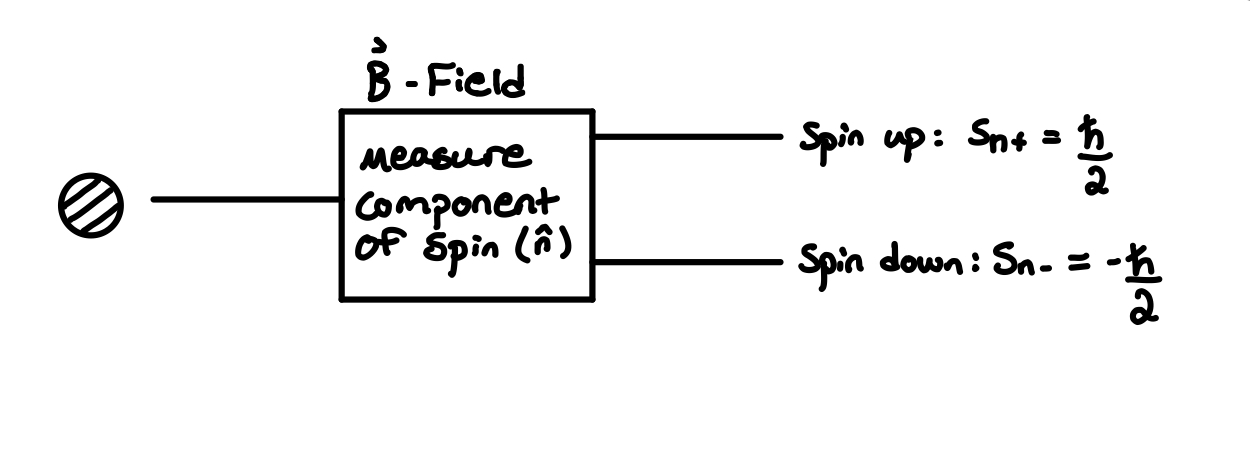
\includegraphics[width=1.00\linewidth]{Spin-In-Magnetic-Field.jpg}
\caption{Measuring any component gives one of two outcomes: $S_{+n}=\hbar/2$ and $S_{-n}=-\hbar/2$. The evolution of this spin - 1/2 particle can be influenced by something like a magnetic field.}
\end{center}
\end{figure}
\newline
A particle that resides in a specific state, usually denoted by $\ket{\psi}$, can be subjected to a measurement influenced by a physical parameter. If we measure $S_{+x}$ we will get $\hbar/2$ with some certainty. The same can be said if we measure $S_{-x}$ we will get $-\hbar/2$ with some certainty. In general we can obtain $\hbar/2$ or $-\hbar/2$ with certainty if we measure in the correct direction depending upon the original orientation of the particle. This can be seen in Figure 2.
%--------------------------------------------------
%	Figure 2
%--------------------------------------------------
\begin{figure}[htbp]
\begin{center}
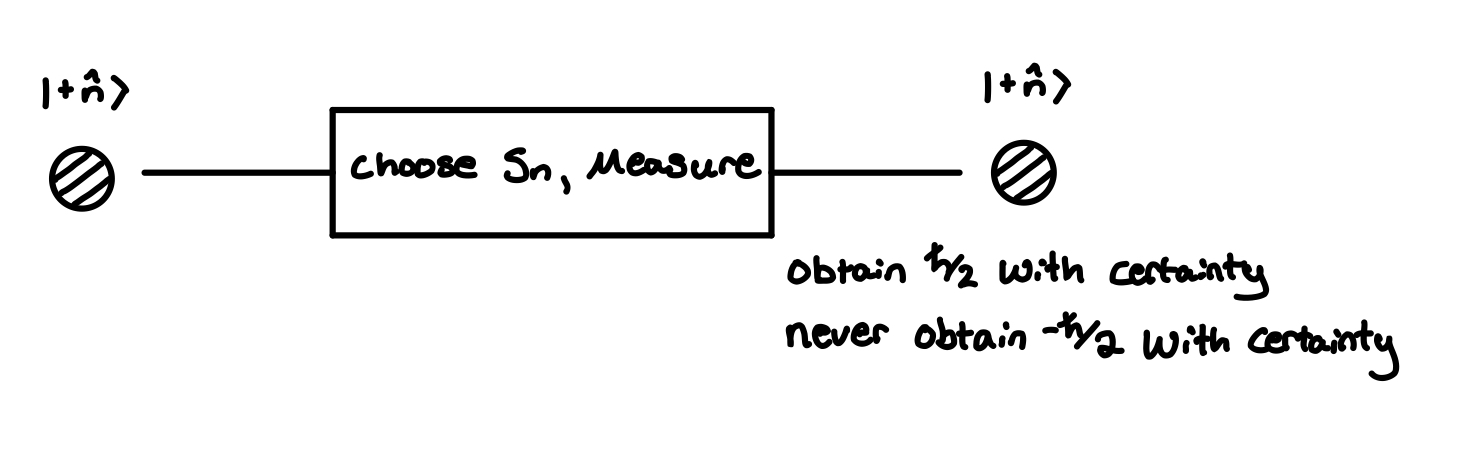
\includegraphics[width=1.00\linewidth]{Spin-With-Certainty.jpg}
\caption{In the schematic above, we have a particle that is originally oriented in the $+\hat{n}$ direction that is being measure in the $+\hat{n}$ direction as well. In this scenario we will never obtain $-\hbar/2$ with some degree of certainty. When the particle is measured the original state that is in is changed to a different final state.}
\end{center}
\end{figure}
\newline
If we now extend the scenario in Figure 2 where we are measuring along the same direction as $\hat{n}$ to measure along a different direction such as $\hat{m}$ we have a different outcome. The schematic of this procedure can be seen in Figure 3.
%--------------------------------------------------
%	Figure 3
%--------------------------------------------------
\begin{figure}[htbp]
\begin{center}
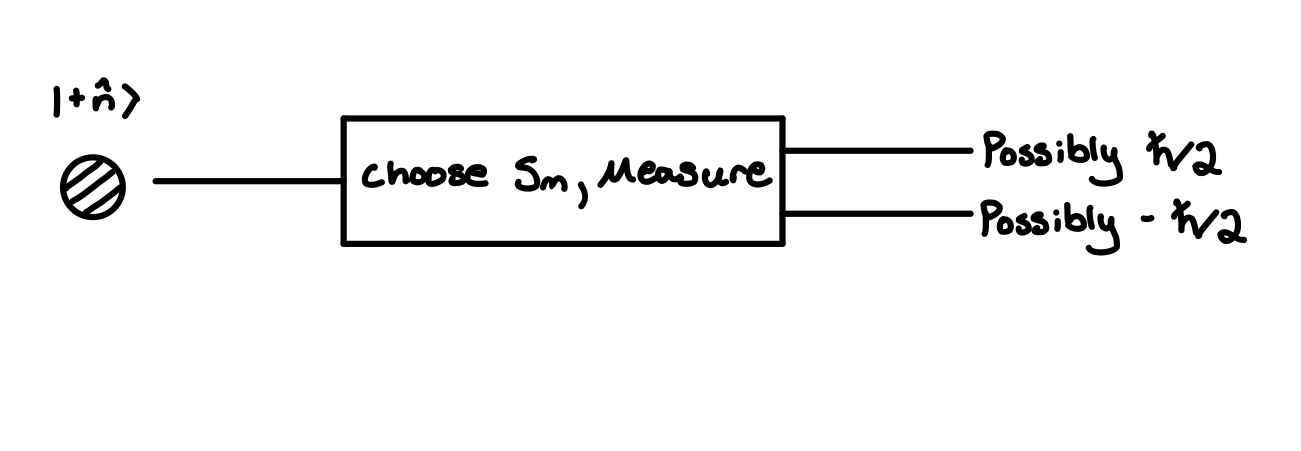
\includegraphics[width=1.00\linewidth]{Spin-With-M-Direction.jpg}
\caption{In this situation it is possible to either obtain $\hbar/2$ or $-\hbar/2$ with some degree of certainty and is largely dependent upon the direction of which we choose to measure along.}
\end{center}
\end{figure}
\newpage
It should also be noted that if we take an exact copy of the state $\ket{+\hat{n}}$ in Figure 3 and repeat the same measurement above we won't necessarily get the same outcome each time. To get a better understanding of the measurement that we are conducting in Figure 3, Figure 4 is created to provide a visual representation.
%--------------------------------------------------
%	Figure 4
%--------------------------------------------------
\begin{figure}[htbp]
\begin{center}
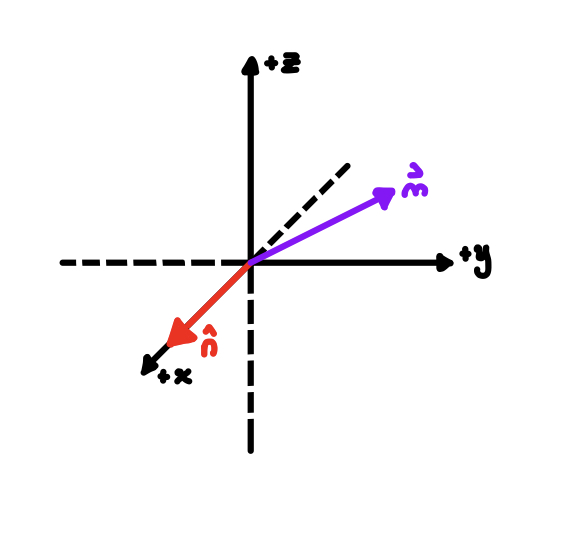
\includegraphics[width=0.75\linewidth]{Spin-With-M-and-N-Graph.jpg}
\caption{This figure is intended to represent how the original state is oriented with respect to the direction that we are measuring with.}
\end{center}
\end{figure}
\newline
Once the measurement in Figure 3 is conducted, we can proceed to calculate the probabilities of obtaining $\hbar/2$ and $-\hbar/2$. The measurements that are depicted in Figure 4 and the outcomes in Figure 3 can be calculated via
%--------------------------------------------------
%	Equation (1)
%--------------------------------------------------
\begin{equation} \label{eq:1}
\bra{\pm n}\ket{\pm m}
\end{equation}
and the probabilities can be calculated via
%--------------------------------------------------
%	Equation (2)
%--------------------------------------------------
\begin{equation} \label{eq:2}
\text{Prob}(S_n=\pm \hbar/2)=|\bra{\pm\hat{n}}\ket{\psi}|^2
\end{equation}
where the probabilities of getting $\hbar/2$ and $-\hbar/2$ must add up to be 1. 

When we take a measurement of states the coefficients follow the rule of $a_0a_0^*+a_1a_1^*=1$. If we have a state $\ket{\psi}$ that follows these rules we can find $\theta$ and $\phi$ such that we can write this state in the $\ket{\pm\hat{n}}$ form. These states in their ket form are
%--------------------------------------------------
%	Equation (3)
%--------------------------------------------------
\begin{align} \label{eq:3}
\ket{\psi}&=a_{+}\ket{+\hat{z}}+a_{-}\ket{-\hat{z}}, \\
\ket{\psi}&=b_{+}\ket{+\hat{z}}+b_{-}\ket{-\hat{z}}. \nonumber
\end{align}
The bra form of these states are represented by
%--------------------------------------------------
%	Equation (4)
%--------------------------------------------------
\begin{align}\label{eq:4}
\bra{\psi}=a_{+}^*\bra{+\hat{z}}+a_{-}^*\bra{-\hat{z}}, \\
\bra{\psi}=b_{+}^*\bra{+\hat{z}}+b_{-}^*\bra{-\hat{z}} \nonumber
\end{align}
and must follow the same rule of $a_0a_0^*+a_1a_1^*=1$. It then follows that $\bra{\psi}\ket{\psi}=b_{+}^*a_{+}+b_{-}^*a_{-}$.

The measuring of states follow certain rules. Take for instance the inner product of a state that is represented by $\ket{\hat{+z}}$. The inner product of $\bra{+\hat{z}}\ket{+\hat{z}}=1$ and more generically the rule follows $\bra{+\hat{n}}\ket{+\hat{n}}=1$ and $\bra{-\hat{n}}\ket{-\hat{n}}=1$. Simultaneously it is also true that $\bra{+\hat{n}}\ket{-\ket{\hat{n}}}=\bra{-\hat{n}}\ket{+\hat{n}}=0$. These rules are valid for any state that is represented by both bras and kets.

The mathematical representation of these $\hat{n}$ states are 
%--------------------------------------------------
%	Equation (5)
%--------------------------------------------------
\begin{equation} \label{eq:5}
\ket{+\hat{n}}=\cos{(\theta/2)}\ket{+\hat{z}}+e^{i\phi}\sin{(\theta/2)}\ket{-\hat{z}}
\end{equation}
and
%--------------------------------------------------
%	Equation (6)
%--------------------------------------------------
\begin{equation} \label{eq:6}
\ket{-\hat{n}}=\sin{(\theta/2)}\ket{+\hat{z}}-e^{i\phi}\cos{(\theta/2)}\ket{-\hat{z}}
\end{equation}
where $\theta$ is the angle of $\hat{n}$ with respect to the $x$-$y$ plane and $\phi$ is the angle off of the $z$ axis. Particles that are subject to being measured can have any orientation with any value of $\theta$ or $\phi$. These angles can either represent the orientation of the initial direction of a particle or how it was affected once we took our measurement. The angles can be seen in Figure 5 \cite{Hazewinkel}.
%--------------------------------------------------
%	Figure 5
%--------------------------------------------------
\begin{figure}[htbp]
\begin{center}
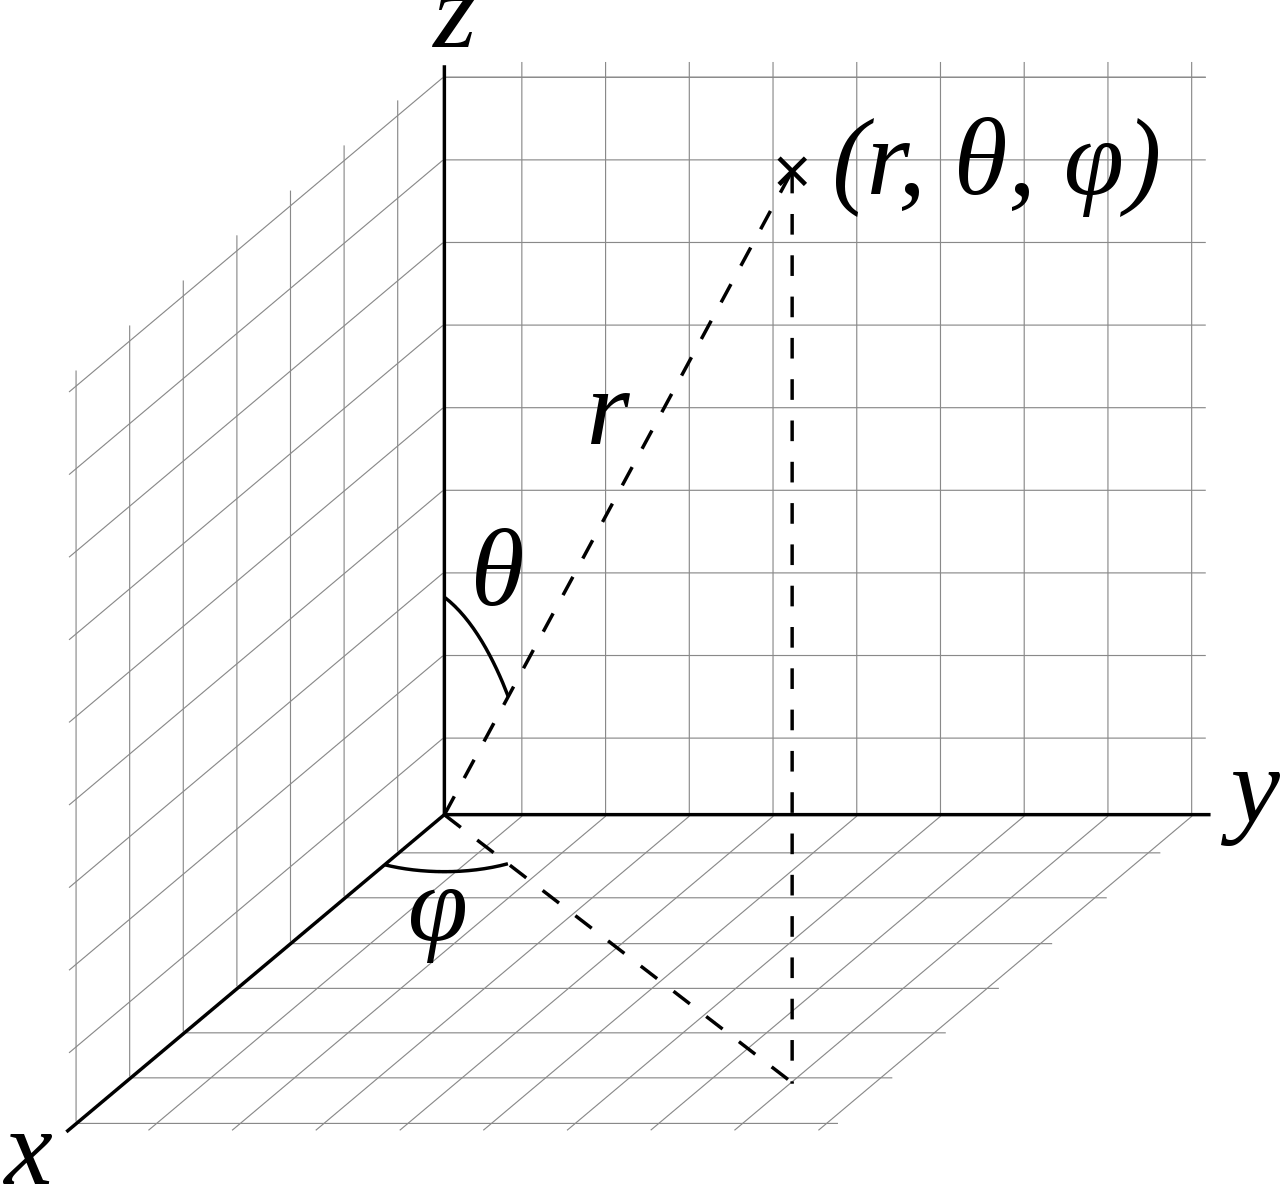
\includegraphics[width=0.75\linewidth]{Spherical-Coordinate-System.png}
\caption{Generic representation of 3D spherical coordinate system.}
\end{center}
\end{figure}
\newpage
With these rules of (\ref{eq:3}), (\ref{eq:4}), (\ref{eq:5}), and (\ref{eq:6}) we originally choose a direction to measure with and we will get one outcome with some probability. This outcome is entirely dependent upon what direction we choose to measure against.

In an experiment you could check this by doing the same process many times and checking the probability. We then begin to have a better understanding of the probability of obtaining $\hbar/2$ or $-\hbar/2$ from our measurement.

Lastly it is more conventional to write equations (\ref{eq:5}) and (\ref{eq:6}) in $\ket{0}$ and $\ket{1}$ notation. Precisely, these equations are
%--------------------------------------------------
%	Equation (7)
%--------------------------------------------------
\begin{equation} \label{eq:7}
\ket{+\hat{n}}=\cos{(\theta/2)}\ket{0}+e^{i\phi}\sin{(\theta/2)}\ket{1}
\end{equation}
and
%--------------------------------------------------
%	Equation (8)
%--------------------------------------------------
\begin{equation} \label{eq:8}
\ket{-\hat{n}}=\sin{(\theta/2)}\ket{0}-e^{i\phi}\cos{(\theta/2)}\ket{1}.
\end{equation}
The notation that is denoted in equation (\ref{eq:7}) and (\ref{eq:8}) is what will be used throughout the rest of this paper to described spin-1/2 particles with specific states.
%---------------------------------------------------------------------------
%	Entangled and Product States
%---------------------------------------------------------------------------
\section*{Entangled and Product States}
We consider how to describe multiple particles. When two particles are being used in a measurement it is essential to understand that each particle will contribute separately to the measurement and will do so simultaneously. When it comes to two particles being used at once there are two kinds of these states: product and entangled states.

Product and entangled states are states that represent multiple particles. Product states are two states of which that can be separated into two separate individual states. Entangled states are states that involve two states that cannot be separated such that each individual state can be recognized. To have a better understanding of how these measurements work a schematic is provided in Figure 6.
%--------------------------------------------------
%	Figure 6
%--------------------------------------------------
\begin{figure}[htpb]
\begin{center}
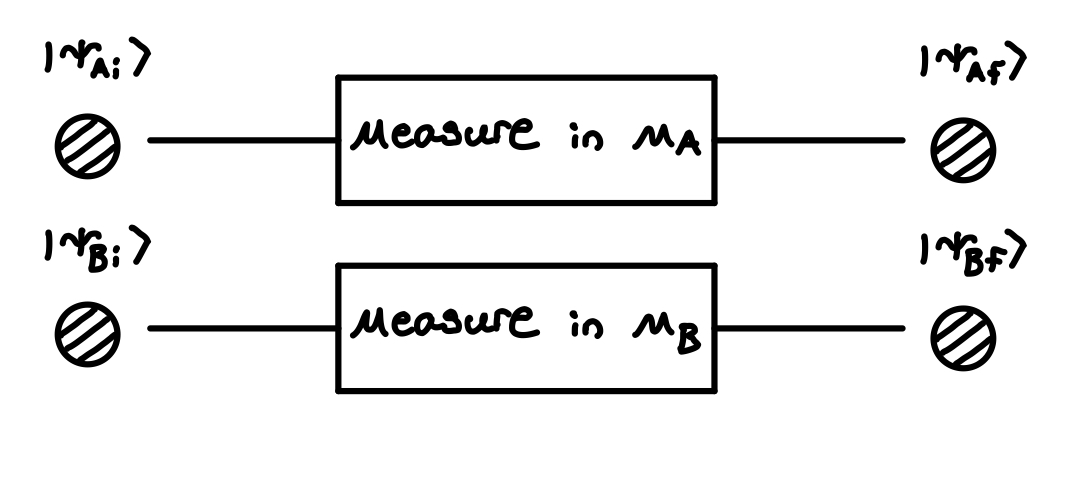
\includegraphics[width=1.00\linewidth]{Two-Particle-Diagram.jpg}
\caption{Example of a two particle measurement scheme.}
\end{center}
\end{figure}
\newline
When these states are being measured like in Figure 6 each state, $\ket{\psi_A}$ and $\ket{\psi_B}$ we have the possibility of either measuring the positive or negative component. The possibilities of measuring these states can be seen in Table 1 for an easier representation.
%--------------------------------------------------
%	Table 1
%--------------------------------------------------
\begin{table}[h!]
\begin{center}
\begin{tabular}{ |c|c|c| }
\hline $\ket{\hat{M}_A}$ & $\ket{\hat{M}_B}$ & \text{State} \\
\hline $+$ & $+$ & $\ket{+\hat{M}_A}\ket{+\hat{M}_B}$ \\
\hline $+$ & $-$ & $\ket{+\hat{M}_A}\ket{-\hat{M}_B}$ \\
\hline $-$ & $+$ & $\ket{-\hat{M}_A}\ket{+\hat{M}_B}$ \\
\hline $-$ & $-$ & $\ket{-\hat{M}_A}\ket{-\hat{M}_B}$ \\
\hline
\end{tabular}
\caption{$\hat{M}$ is the direction of which we choose to measure. The ``+" and ``-" indicate what the possibilities are for each particle that is being measured.}
\end{center}
\end{table} 
\newline
Take for instance measuring the $z$ component of each spin-$1/2$ particle. Within these multiple particle states there are a set of generic states. These generic states are $\ket{0}\ket{0}$, $\ket{0}\ket{1}$, $\ket{1}\ket{0}$, and $\ket{1}\ket{1}$. In these generic states we have a combination of particles either being positive or negative. The $\ket{0}$'s are positive and the $\ket{1}$'s are negative. If the state is in $\ket{0}\ket{0}$ initially, we will get $+$ for both $A$ and $B$. If the state is in $\ket{0}\ket{1}$ initially, we will get $+$ for $A$ and $-$ for $B$. With the state being in $\ket{1}\ket{0}$, we will get $-$ for $A$ and $+$ for $B$. Lastly, if the state is in $\ket{1}\ket{1}$, we will get $-$ for both $A$ and $B$.

The generic representation of these states is
%--------------------------------------------------
%	Equation (9)
%--------------------------------------------------
\begin{equation}\label{eq:9}
\ket{\psi}=c_0\ket{0}\ket{0}+c_1\ket{0}\ket{1}+c_2\ket{1}\ket{0}+c_3\ket{1}\ket{1}
\end{equation}
where $c_0$, $c_1$, $c_2$, and $c_3$ are all numeric coefficients for these these states. Within these dual particle states there are states of which are entangled or product states where we can take measurements and calculate probabilities. The way these probabilities are calculated is
%--------------------------------------------------
%	Equation (10)
%--------------------------------------------------
\begin{equation}\label{eq:10}
\text{Prob}=|\bra{n_{0,1}}\bra{n_{0,1}}\ket{\psi}|^2
\end{equation}
where $\bra{n_0}=\bra{0}$ and $\bra{n_1}=\bra{1}$. For instance, if the state that we are measuring is originally in $\bra{0}\bra{1}$ and our measurement is $\bra{0}\bra{1}\ket{\psi}$, this means that we are measuring $\ket{\psi}$ when state A is positive and state B is negative. This calculation follows the scheme of what is seen in equation (\ref{eq:1}) but with two particles instead of just one.

Take for instance a product state that can be represented by
%--------------------------------------------------
%	Equation (11)
%--------------------------------------------------
\begin{equation}\label{eq:11}
\ket{\psi}=\ket{\psi_A}\ket{\psi_B}
\end{equation}
where equation (\ref{eq:11}) can be written as a combination of states such that
%--------------------------------------------------
%	Equation (12)
%--------------------------------------------------
\begin{equation}\label{eq:12}
\ket{\psi}=\frac{1}{2}\big(\ket{0}\ket{0}+\ket{0}\ket{1}-\ket{1}\ket{0}-\ket{1}\ket{1}\big).
\end{equation}
This means that this state consists of two states that are each individually their own state. Just as equation (\ref{eq:11}) represents a product state, entangled states can be written in a similar fashion. An example of an entangled state is
%--------------------------------------------------
%	Equation (13)
%--------------------------------------------------
\begin{equation}\label{eq:13}
\ket{\psi}=\frac{1}{2}\big(\ket{0}\ket{0}+\ket{0}\ket{1}+\ket{1}\ket{0}-\ket{1}\ket{1}\big).
\end{equation}
Equation (\ref{eq:13}) cannot be separated into two separate states in the form of equation (\ref{eq:11}) and this is what makes the state entangled. We cannot come up with a $\ket{\psi_A}$ and $\ket{\psi_B}$ for this specific entangled state.
%---------------------------------------------------------------------------
%	Unitary Operators
%---------------------------------------------------------------------------
\section*{Unitary Operators}
The evolution of a state such as a particle entering a magnetic field will now be discussed. Figure 7 depicts an elementary evolution of a state.
%--------------------------------------------------
%	Figure 7
%--------------------------------------------------
\begin{figure}[htpb]
\begin{center}
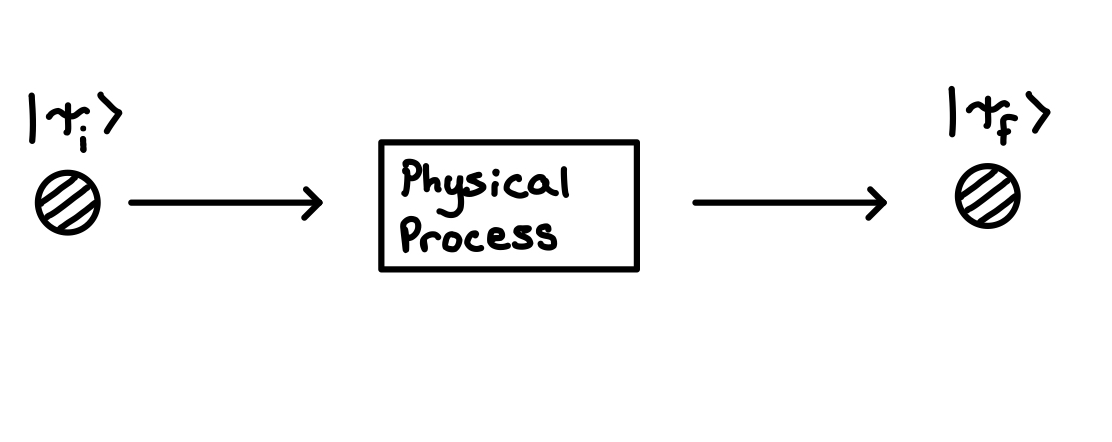
\includegraphics[width=0.90\linewidth]{Unitary-Operator.PNG}
\caption{Schematic of a unitary operator.}
\end{center}
\end{figure}\\
Mathematically the evolution of a state can be calculated by
%--------------------------------------------------
%	Equation (14)
%--------------------------------------------------
\begin{equation}\label{eq:14}
\ket{\psi_f}=\hat{U}\ket{\psi_i}
\end{equation}
where $\hat{U}^{\dagger}\hat{U}=\hat{I}$ must be true. These linear operators are also called unitary operators.  The $\hat{U}$ in equation (\ref{eq:14}) is a unitary operator. As an example, consider 
%--------------------------------------------------
%	Equation (15)
%--------------------------------------------------
\begin{equation}\label{eq:15}
\hat{U}=
\begin{pmatrix}
1 & 0 \\
0 & -1
\end{pmatrix}.
\end{equation}
The effects of the unitary operator represented by equation (\ref{eq:15}) acting on specific initial states can be seen in Table 2.
%--------------------------------------------------
%	Table 2
%--------------------------------------------------
\begin{table}[h!]
\begin{center}
\begin{tabular}{ |c|c| }
\hline $\ket{\psi_i}$& $\hat{U}\ket{\Psi_i}=\ket{\psi_f}$ \\
\hline $\ket{0}$& $\ket{0}$\\
\hline $\frac{1}{\sqrt{2}}\big(\ket{0}+\ket{1}\big)$& $\frac{1}{\sqrt{2}}\big(\ket{0}-\ket{1}\big)$\\
\hline $\frac{1}{2}\big(\ket{0}+i\ket{1}\big)$& $\frac{1}{\sqrt{2}}\big(\ket{0}-i\ket{1}\big)$\\
\hline
\end{tabular}
\caption{Effect of a unitary operator, equation (\ref{eq:14}) acting on spin-$1/2$ particle.}
\end{center}
\end{table}
\newline 
When the unitary operator in equation (\ref{eq:15}) acts on the spin-1/2 particles in Table 1 it subsequently rotates the direction that it was originally oriented in. For instance, these rotations are occurring about the $z$ axis. The state that is originally in the $+x$ direction rotates to the $-x$ direction. Conversely the $+y$ orientation shifts to the $-y$. The particle that is oriented originally in the $\pm z$ direction is unaffected and remains the same after the evolution. These shifts can be seen in Table 3.
%--------------------------------------------------
%	Table 3
%--------------------------------------------------
\begin{table}[h!]
\begin{center}
\begin{tabular}{ |c|c|c|c| }
\hline $\ket{\psi_i}$ $(\theta_i)$& $\ket{\psi_i}$ $(\phi_i)$& $\ket{\psi_f}$ $(\theta_f)$& $\ket{\psi_f}$ $(\psi_f)$ \\
\hline 0 & 0 & 0 & 0 \\
\hline $\pi/2$ & 0 & $\pi/2$ & $\pi$ \\
\hline $\pi/2$ & $\pi/2$ & $\pi/2$ & $3\pi/2$ \\
\hline
\end{tabular}
\caption{The effect of equation (\ref{eq:15}) on the $\theta$ and $\phi$ angles.}
\end{center}
\end{table}
\newline
The rows in Table 3 are angles in radians for each state previously mentioned in Table 2. It can be observed that the $\theta$ angle is not affected by the unitary operator acting on the spin-1/2 particles in these specific original states. Instead, when the spin-1/2 particle is originally oriented in the $x$ or $y$-direction the $\phi$ angle is reoriented by an angle of $\pi$. This is because this unitary operator is causing a rotation for these particles about the $z$ axis. This rotation about the $z$ axis is why the particle that is originally oriented in the $z$ direction (The first row of Table 3) is unaffected by this unitary operator in equation (\ref{eq:15}).

There are also special unitary operators called Pauli operators and there is one Pauli operator for the $x$, $y$, and $z$-direction. The Pauli operators are
%--------------------------------------------------
%	Equation (16)
%--------------------------------------------------
\begin{equation}\label{eq:16}
\hat{\sigma}_x=
\begin{pmatrix}
0 & 1 \\
1 & 0
\end{pmatrix},
\end{equation}
%--------------------------------------------------
%	Equation (17)
%--------------------------------------------------
\begin{equation}\label{eq:17}
\hat{\sigma}_y=
\begin{pmatrix}
0 & -i \\
i & 0
\end{pmatrix},
\end{equation}
and
%--------------------------------------------------
%	Equation (18)
%--------------------------------------------------
\begin{equation}\label{eq:18}
\hat{\sigma}_z=
\begin{pmatrix}
1 & 0 \\
0 & -1
\end{pmatrix}.
\end{equation}
Similar to unitary operators, Pauli operators all follow a certain list of specific rules. The first rule is that any Pauli operator in any direction multiplied with itself will yield the identity matrix. Mathematically this can be interpreted as
%--------------------------------------------------
%	Equation (19)
%--------------------------------------------------
\begin{equation}\label{eq:19}
\hat{\sigma_n}^2=\hat{I}
\end{equation}
where $n$ is either the $x$, $y$, or $z$-direction. The next rule is for when we multiply separate Pauli operators in different directions we get something of the form $i\sigma_n$. Particularly these rules are
%--------------------------------------------------
%	Equation (20)
%--------------------------------------------------
\begin{equation}\label{eq:20}
\hat{\sigma}_x\hat{\sigma}_y=i\hat{\sigma}_z,
\end{equation}
%--------------------------------------------------
%	Equation (21)
%--------------------------------------------------
\begin{equation}\label{eq:21}
\hat{\sigma}_y\hat{\sigma}_z=i\hat{\sigma}_x,
\end{equation}
%--------------------------------------------------
%	Equation (22)
%--------------------------------------------------
\begin{equation}\label{eq:22}
\hat{\sigma}_z\hat{\sigma}_x=i\hat{\sigma}_y,
\end{equation}
and
%--------------------------------------------------
%	Equation (23)
%--------------------------------------------------
\begin{equation}\label{eq:23}
\hat{\sigma}_x\hat{\sigma}_y=-\hat{\sigma}_y\hat{\sigma}_x.
\end{equation}
The last rule is
%--------------------------------------------------
%	Equation (24)
%--------------------------------------------------
\begin{equation}\label{eq:24}
\sigma^2=\big(n_x^2+n_y^2+n_z^2\big)\hat{I}
\end{equation}
where
%--------------------------------------------------
%	Equation (25)
%--------------------------------------------------
\begin{equation}\label{eq:25}
\hat{\sigma}_n=n_x\hat{\sigma}_x+n_y\hat{\sigma}_y+n_z\hat{\sigma}_z
\end{equation}
with $n_x$, $n_y$, and $n_z$ all being constants. With these rules we can drastically simplify our math when dealing with these Pauli operators.

These Pauli operators will be referenced later in this paper and instead of writing out a matrix every time they are mentioned we will just refer to these equations.
%---------------------------------------------------------------------------
%	Unitary Operators With a Parameter
%---------------------------------------------------------------------------
\section*{Unitary Operators With a Parameter}
Unitary operators can describe physical evolutions that are dependent upon parameters. Take for instance the unitary operator
%--------------------------------------------------
%	Equation (26)
%--------------------------------------------------
\begin{equation}\label{eq:26}
\hat{U}(\lambda)=
\begin{pmatrix}
e^{-i\lambda/2} & 0 \\
0 & e^{i\lambda/2}
\end{pmatrix}
\end{equation}
which is dependent upon the parameter $\lambda$. When this unitary operator acts on states it will produce a final state after that is also dependent upon a parameter. The results of this unitary operator acting on specific spin-1/2 states can be seen in Table 4.
\newpage
%--------------------------------------------------
%	Table 4
%--------------------------------------------------
\begin{table}[h!]
\begin{center}
\begin{tabular}{ |c|c| }
\hline $\ket{\psi_i}$& $\hat{U}\ket{\Psi_i}=\ket{\psi_f}$ \\
\hline $\ket{0}$& $e^{-i\lambda/2}\ket{0}$\\
\hline $\frac{1}{\sqrt{2}}\big(\ket{0}+\ket{1}\big)$& $\frac{1}{\sqrt{2}}\big(e^{-i\lambda/2}\ket{0}+e^{i\lambda/2}\ket{1}\big)$\\
\hline $\frac{1}{5}\big(4\ket{0}+3\ket{1}\big)$& $\frac{1}{5}\big(4e^{-i\lambda/2}\ket{0}+3e^{i\lambda/2}\ket{1}\big)$\\
\hline
\end{tabular}
\caption{Effect of the unitary operator $\hat{U}(\lambda)$, equation ($\ref{eq:26}$), on initial spin-1/2 particle states.}
\end{center}
\end{table} 

Using the $\ket{\psi_f}$ states and comparing them with $\ket{\psi_i}$ we can see how the unitary operator affected the original state. These effects can be seen in Table 5.
%--------------------------------------------------
%	Table 5
%--------------------------------------------------
\begin{table}[h!]
\begin{center}
\begin{tabular}{ |c|c|c|c| }
\hline $\ket{\psi_i}$ $(\theta_i)$& $\ket{\psi_i}$ $(\phi_i)$& $\ket{\psi_f}$ $(\theta_f)$& $\ket{\psi_f}$ $(\phi_f)$ \\
\hline 0 & 0 & 0 & 0 \\
\hline $\pi/2$ & 0 & $\pi/2$ & $\lambda$ \\
\hline $73.7\degree$ & $0$ & $73.7\degree$ & $\lambda$ \\
\hline
\end{tabular}
\caption{Effect of the unitary operator $\hat{U}(\lambda)$, equation ($\ref{eq:26}$), on the $\theta$ and $\phi$ angles.}
\end{center}
\end{table} \\
What happens to these states geometrically is that when a particle is originally in the state $\ket{\psi_i}$ it will be mapped to $\ket{\psi_f}$. In the context of this example the $\theta$ angles of the second and third states are unaffected where the $\phi$ angle is being rotated by the angle $\lambda$. 

Another way of writing unitary operators is with the use of matrix exponentials. This can be done using the formula
%--------------------------------------------------
%	Equation (27)
%--------------------------------------------------
\begin{equation}\label{eq:27}
e^{-i\lambda\hat{\sigma}_n}=\cos{(\lambda)}\hat{I}-i\sin{(\lambda)}\hat{\sigma_n}.
\end{equation}
For example, $e^{-i\lambda\hat{\sigma}_z}$ can be written in the matrix form
%--------------------------------------------------
%	Equation (28)
%--------------------------------------------------
\begin{equation}\label{eq:28}
e^{-i\lambda\hat{\sigma}_z}=
\begin{pmatrix}
\cos{(\lambda)}-i\sin{(\lambda)} & 0 \\
0 & \cos{(\lambda)}+i\sin{(\lambda)}
\end{pmatrix}.
\end{equation}
This is a more compact way to represent this matrix with $e^{-i\lambda\hat{\sigma}_z}$.
%---------------------------------------------------------------------------
%	Two Qubit Unitary Operators
%---------------------------------------------------------------------------
\section*{Two Qubit Unitary Operators}
It is also necessary to describe the evolution of multiple particles. Consider two qubits, schematically these two qubit unitary operators can be thought of as what is pictured in Figure 8.
%--------------------------------------------------
%	Figure 8
%--------------------------------------------------
\begin{figure}[htpb]
\begin{center}
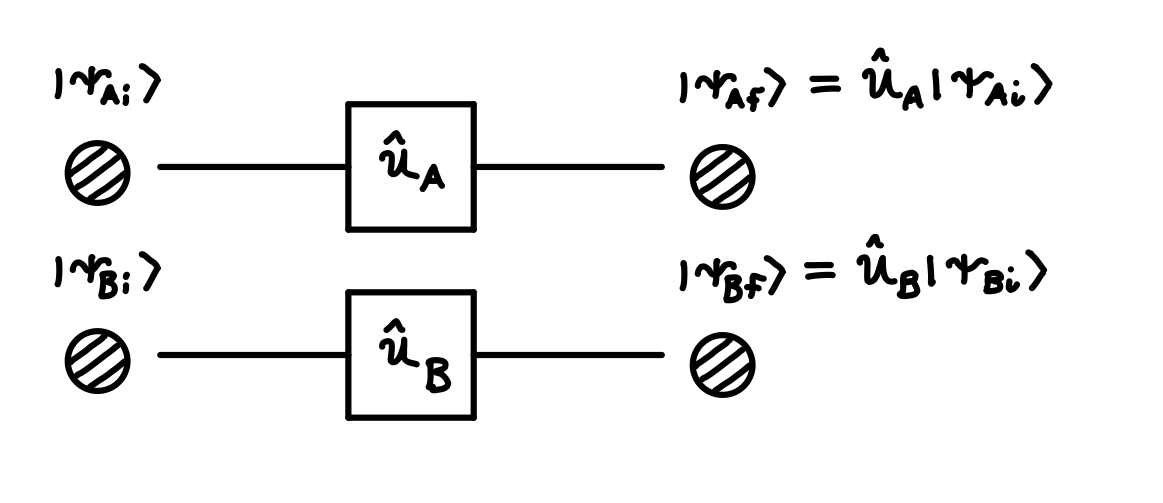
\includegraphics[width=0.90\linewidth]{Two-Qubit-Unitary-Schematic.jpg}
\caption{A schematic of a particular type of a two qubit unitary operator. $\hat{U}_A$ and $\hat{U}_B$ are unitary operators that each represent a specific particle evolution.}
\end{center}
\end{figure}\\
These two qubit unitary operators consist of two $2\times2$ unitaries. Two qubit unitary operators can be calculated via a tensor product. The tensor product of two matrices is
%--------------------------------------------------
%	Equation (29)
%--------------------------------------------------
\begin{equation} \label{eq:29}
\hat{A}\otimes\hat{B}=
\left(\begin{array}{cccc}
a_1b_1 & a_1b_2 & a_2b_1 & a_2b_2 \\
a_1b_3 & a_1b_4 & a_2b_3 & a_2b_4 \\
a_3b_1 & a_3b_2 & a_4b_1 & a_4b_2 \\
a_3b_3 & a_3b_4 & a_4b_3 & a_4b_4 \\
\end{array}\right).
\end{equation}
Consider for instance the two evolution operators
%--------------------------------------------------
%	Equation (30)
%--------------------------------------------------
\begin{equation} \label{eq:30}
\hat{U}_A=
\begin{pmatrix}
e^{-i\alpha/2} & 0 \\
0 & e^{i\alpha/2}
\end{pmatrix}
\end{equation}
and
%--------------------------------------------------
%	Equation (31)
%--------------------------------------------------
\begin{equation} \label{eq:31}
\hat{U}_B=
\begin{pmatrix}
e^{-i\beta/2} & 0 \\
0 & e^{i\beta/2}
\end{pmatrix}.
\end{equation}
Taking the tensor product of the matrices in equation (\ref{eq:30}) and (\ref{eq:31}) we get
%--------------------------------------------------
%	Equation (32)
%--------------------------------------------------
\begin{equation} \label{eq:32}
\left(\begin{array}{cccc}
e^{-i(\alpha+\beta)/2} & 0 & 0 & 0 \\
0 & e^{i(\beta-\alpha)/2} & 0 & 0 \\
0 & 0 & e^{i(\alpha-\beta)/2} & 0 \\
0 & 0 & 0 & e^{i(\alpha+\beta)/2} \\
\end{array}\right)
\end{equation}
as what is called a joint operator. These two qubit unitary operators will be discussed more thoroughly in the pursuit of determining a parameter. This joint operator describes the evolution of a two qubit state such as the one seen in equation (\ref{eq:9}).

In the presence of two qubits interacting the evolution has to be described by an operator that acts on a pair of qubits. A common qubit unitary that behaves in this manner is called the controlled-NOT gate and is denoted $\hat{U}_{CNOT}$. This matrix is abbreviated by $\hat{U}_{\tiny{CNOT}}$ and is
%--------------------------------------------------
%	Equation (33)
%--------------------------------------------------
\begin{equation} \label{eq:33}
\hat{U}_{\tiny{CNOT}}=
\left(\begin{array}{cccc}
1 & 0 & 0 & 0 \\
0 & 1 & 0 & 0 \\
0 & 0 & 0 & 1 \\
0 & 0 & 1 & 0 \\
\end{array}\right)
\end{equation}
and has the ability to change a product state to an entangled state for given initial states. The evolution of specific states under the controlled not unitary operator can be seen in Table 6.
%--------------------------------------------------
%	Table 6
%--------------------------------------------------
\begin{table}[h!]
\begin{center}
\begin{tabular}{ |c|c|c| }
\hline $\ket{\psi_0}$ & $\hat{U_{CNOT}}\ket{\Psi_0}=\ket{\psi}$ & Result \\
\hline $\frac{1}{\sqrt{2}}(\ket{0}\ket{0}+\ket{0}\ket{1})$ & $\frac{1}{\sqrt{2}}(\ket{0}\ket{0}+\ket{0}\ket{1})$ & Prod. \\
\hline $\frac{1}{\sqrt{2}}(\ket{0}\ket{0}+\ket{1}\ket{0})$ & $\frac{1}{\sqrt{2}}(\ket{0}\ket{0}+\ket{1}\ket{1})$ & Ent. \\
\hline $\frac{1}{\sqrt{2}}(\ket{0}\ket{0}+\ket{1}\ket{1})$ & $\frac{1}{\sqrt{2}}(\ket{0}\ket{0}+\ket{1}\ket{0})$ & Prod. \\
\hline $\frac{1}{\sqrt{2}}(\ket{0}\ket{1}+\ket{1}\ket{0})$ & $\frac{1}{\sqrt{2}}(\ket{0}\ket{1}+\ket{1}\ket{1})$ & Prod. \\
\hline 
\end{tabular}
\caption{Effect of the controlled not operator acting on original product and entangled states.}
\end{center}
\end{table} \\
As observed in Table 6, sometimes the controlled-NOT operator converts a product state to an entangled state and vice versa.
%---------------------------------------------------------------------------
%	Density Operators
%---------------------------------------------------------------------------
\section*{Density Operators}
The next type of operator that we will examine is a density operator. With density operators we do not specifically know the state of the particle with certainty. Also with density operators we only know $\ket{\psi_1}$ with probability $a_1$ and $\ket{\psi_2}$ and probability $a_2$. With this information one can calculate probabilities of measurement outcomes. 

Mathematically these density operators can be calculated by
%--------------------------------------------------
%	Equation (34)
%--------------------------------------------------
\begin{equation} \label{eq:34}
\hat{\rho}=a_1\ket{\psi_1}\bra{\psi_1}+a_2\ket{\psi_2}\bra{\psi_2}.
\end{equation}
For instance, if we know that the initial state is $\ket{0}$ with the probability of $q$ and $\ket{1}$ with the probability of $1-q$, the respective density operator $\hat{\rho}$ is
%--------------------------------------------------
%	Equation (35)
%--------------------------------------------------
\begin{equation} \label{eq:35}
\hat{\rho}=
\begin{pmatrix}
q & 0 \\
0 & 1-q
\end{pmatrix}.
\end{equation}
A pure state is tif the state of the system can be described by a ket $\ket{\psi}$ and is calculated via $\hat{\rho}=\ket{\psi}\bra{\psi}$. In the case of pure states one can show that $\hat{\rho}^2=\hat{\rho}$. If the state is not a pure state the density operator cannot be written as $\hat{\rho}^2=\hat{\rho}$. 

The way we calculate the probability of a measurement outcome is
%--------------------------------------------------
%	Equation (36)
%--------------------------------------------------
\begin{equation} \label{eq:36}
\text{Probability}=Tr[\hat{\rho}\hat{\Pi}]
\end{equation}
where the trace of a matrix, $Tr$, is defined as the addition of the diagonals of a matrix. In equation (\ref{eq:36}) $\hat{\Pi}_0$ is a measurement operator for a given direction. The way these two measurement operators measure something like $S_n$ are calculated via
%--------------------------------------------------
%	Equation (37)
%--------------------------------------------------
\begin{equation}\label{eq:37}
\hat{\Pi}_{+n}=\ket{+\hat{n}}\bra{+\hat{n}}
\end{equation}
and
%--------------------------------------------------
%	Equation (38)
%--------------------------------------------------
\begin{equation}\label{eq:38}
\hat{\Pi}_{-n}=\ket{-\hat{n}}\bra{-\hat{n}}.
\end{equation}
Equation (\ref{eq:37}) represents if we are measuring the $S_+$ direction and equation (\ref{eq:38}) represents the measurement of $S_-$.

An example of how these measurement operators are used can be done with a density operator. Take for instance the density operator
%--------------------------------------------------
%	Equation (39)
%--------------------------------------------------
\begin{equation} \label{eq:39}
\hat{\rho}=\frac{1}{2}
\begin{pmatrix}
1 & r \\
r & 1
\end{pmatrix}
\end{equation}
where we wish to calculate the probability of measuring $\hbar/2$ and $-\hbar/2$ for the $x$ and $y$-directions. A schematic of how these measurement operators work can be seen in Figure 9.
%--------------------------------------------------
%	Figure 9
%--------------------------------------------------
\begin{figure}[h]
\begin{center}
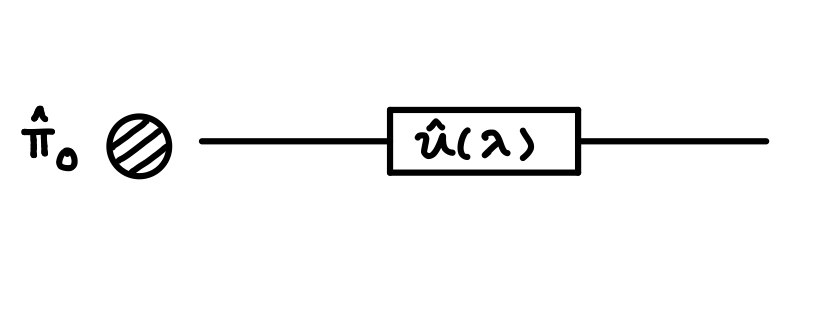
\includegraphics[width=0.90\linewidth]{Density-Operator-Evolution.jpg}
\caption{Evolution of a single qubit density operator evolution.}
\end{center}
\end{figure}
It should be noted that $r$ ranges between 0 and 1. The measurement operator for the positive $x$-direction is
%--------------------------------------------------
%	Equation (40)
%--------------------------------------------------
\begin{equation} \label{eq:40}
\hat{\Pi}_{+x}=\frac{1}{2}
\begin{pmatrix}
1 & 1 \\
1 & 1
\end{pmatrix}
\end{equation}
and the negative $x$-direction is
%--------------------------------------------------
%	Equation (41)
%--------------------------------------------------
\begin{equation} \label{eq:41}
\hat{\Pi}_{-x}=\frac{1}{2}
\begin{pmatrix}
1 & -1 \\
-1 & 1
\end{pmatrix}.
\end{equation}
The measurement operator for the positive $y$-direction is
%--------------------------------------------------
%	Equation (42)
%--------------------------------------------------
\begin{equation} \label{eq:42}
\hat{\Pi}_{+y}=\frac{1}{2}
\begin{pmatrix}
1 & -i \\
i & 1
\end{pmatrix}
\end{equation}
and the negative $y$-direction is
%--------------------------------------------------
%	Equation (43)
%--------------------------------------------------
\begin{equation} \label{eq:43}
\hat{\Pi}_{-y}=\frac{1}{2}
\begin{pmatrix}
1 & i \\
-i & 1
\end{pmatrix}.
\end{equation}
Using equation (\ref{eq:36}) we can calculate the probabilities for both of these directions. The results for these calculations can be seen in Table 7.
%--------------------------------------------------
%	Table 7
%--------------------------------------------------
\begin{table}[h!]
\begin{center}
\begin{tabular}{ |c|c| }
\hline Direction & Probability \\
\hline Tr[$\hat{\rho}\hat{\rho}_{+x}$] & $\frac{1}{2}(1+r)$ \\
\hline Tr[$\hat{\rho}\hat{\rho}_{-x}$] & $\frac{1}{2}(1-r)$ \\
\hline Tr[$\hat{\rho}\hat{\rho}_{+y}$] & $\frac{1}{2}$ \\
\hline Tr[$\hat{\rho}\hat{\rho}_{-y}$] & $\frac{1}{2}$ \\
\hline
\end{tabular} 
\caption{Probabilities of measuring $\hbar/2$ and $-\hbar/2$ with the $x$ and $y$-direction density operatorsas defined in equations (\ref{eq:39}) through (\ref{eq:43}).}
\end{center}
\end{table}
\newline 
Under a physical process, the density operator must evolve. This is given by
%--------------------------------------------------
%	Equation (44)
%--------------------------------------------------
\begin{equation} \label{eq:44}
\hat{\rho}(\lambda)=\hat{U}(\lambda)\hat{\rho}_0\hat{U}^{t}(\lambda).
\end{equation}

Using the density operator in equation (\ref{eq:39}) with the unitary operator
%--------------------------------------------------
%	Equation (45)
%--------------------------------------------------
\begin{equation} \label{eq:45}
\hat{U}(\lambda)=
\begin{pmatrix}
e^{-i\lambda/2} & 0 \\
0 & e^{i\lambda/2}
\end{pmatrix}
\end{equation}
the result of equation (\ref{eq:44}) is
%--------------------------------------------------
%	Equation (46)
%--------------------------------------------------
\begin{equation} \label{eq:46}
\hat{\rho}(\lambda)=\frac{1}{2}
\begin{pmatrix}
1 & re^{-i\lambda} \\
re^{i\lambda} & 1
\end{pmatrix}.
\end{equation}
The result from equation (\ref{eq:46}) shows that a unitary that is dependent upon a parameter can produce a density operator that is dependent upon a parameter.
%---------------------------------------------------------------------------
%	Fisher Information
%---------------------------------------------------------------------------
\section*{Fisher Information}
When estimating parameters we assume that there is a known process that depends upon and unknown parameter. The example of a coin flip experiment is an example that illustrates issues in classical estimation. One wants to estimate the parameter by subjecting physical systems to a process followed by measurements. Once these measurements are taken one can infer the parameter from these measurements. When this physical process is repeated there will be different outcomes due to statistical fluctuations. One such example of this is a coin flip experiment.

Consider a coin flip experiment where the only possible outcomes are heads or tails. In this experiment we are interested in finding the probability estimate of how often we will obtain heads. There is a probability of how often someone gets heads in this experiment represented by $P$. This value of $P$ is unknown and is the goal of what we want to estimate. One would flip the coin $N$ number of times. Then the number of times that heads occurs will be recorded as $n_H$. Mathematically, the probability estimate can be calculated via
%--------------------------------------------------
%	Equation (47)
%--------------------------------------------------
\begin{equation}\label{eq:47}
P_{\text{est}}=\frac{n_H}{N}.
\end{equation}
After many calculations with the use of statistical rules and runs of the same experiment we can determine that
%--------------------------------------------------
%	Equation (48)
%--------------------------------------------------
\begin{equation} \label{eq:48}
\bar{P}_{est}=P
\end{equation}
which means that after many trials we should expect to see that our average probability estimate will equal the probability itself. The variance can be calculated via
%--------------------------------------------------
%	Equation (49)
%--------------------------------------------------
\begin{equation} \label{eq:49}
\nu=\bar{P}^2_{est}-(\bar{P}_{est})^2.
\end{equation}
and quantifies the fluctuation in our estimate. In the context of a coin flip experiment the variance can be calculated to be
%--------------------------------------------------
%	Equation (50)
%--------------------------------------------------
\begin{equation} \label{eq:50}
\nu=\frac{P}{N}(1-P)
\end{equation}
where P is the probability of getting heads and N is the number of times that the experiment is ran. The larger value of N, or how many times the experiment is conducted, the smaller variance we will obtain in the experiment. 

The estimate improves with a higher number of trials and one can estimate in many ways using $N$ and $n_H$. We then begin to ask which would be best. We can show that regardless of estimation choice the best that one can do is
%--------------------------------------------------
%	Equation (51)
%--------------------------------------------------
\begin{equation} \label{eq:51}
\nu(P_{est})\geq\frac{1}{F_{\text{\footnotesize{N Toss}}}}
\end{equation}
\cite{D. Collins}. The Fisher Information bounds the variance of a measurement.  The variance decreases with a higher Fisher Information value. A smaller variance means a more precise measurement.

The formula for how the Fisher Information is calculated is 
%--------------------------------------------------
%	Equation (52)
%--------------------------------------------------
\begin{equation} \label{eq:52}
F=\Sigma\frac{1}{\text{\footnotesize{P(Outcome)}}}\Big(\frac{\partial \text{\footnotesize{P(Outcome)}}}{\partial\text{\footnotesize{Parameter}}}\Big)^2
\end{equation}
where $\text{P(Outcome)}$ is a probability that is calculated in the measurement procedure \cite{Paris}. In the context of a coin flip experiment where the only two possible outcomes are heads or tails the Fisher Information of N number of tosses is
%--------------------------------------------------
%	Equation (53)
%--------------------------------------------------
\begin{equation} \label{eq:53}
F_{\text{\footnotesize{N Toss}}}=N\cdot F=\frac{N}{P(1-P)}.
\end{equation}
Equation (\ref{eq:53}) represents the simplest example of the Fisher Information that can be used in an experiment with a finite number of possible outcomes. Once the probabilities within a measurement are calculated we can proceed to run them through equation (\ref{eq:52}) and then add all of these results together at the end. In the context of this coin flip experiment the Fisher Information eliminates the choice of what to do with $n_H$.
%---------------------------------------------------------------------------
%	Fisher Information of Product and Entangled States
%---------------------------------------------------------------------------
\section*{Fisher Information of Product and Entangled States}
The Fisher Information depends on probabilities of measurements. The probabilities of measurements depend on the choice of the measurement. For example if the measurement is done in $x$ or $z$ direction. The question that arises is what measurement gives the greatest Fisher Information. 

For example consider estimating the parameter $\lambda$ in the phase shift of equation(\ref{eq:54})
%--------------------------------------------------
%	Equation (54)
%--------------------------------------------------
\begin{equation} \label{eq:54}
\hat{U}(\lambda)=
\begin{pmatrix}
e^{-i\lambda/2} & 0 \\
0 & e^{i\lambda/2}
\end{pmatrix}.
\end{equation}
This evolution operator acts on a spin-$1/2$ particle in the initial state
%--------------------------------------------------
%	Equation (55)
%--------------------------------------------------
\begin{equation} \label{eq:55}
\ket{\psi_i}=\frac{1}{\sqrt{2}}\big(\ket{0}\ket{0}+\ket{0}\ket{1}+\ket{1}\ket{0}+\ket{1}\ket{1}\big)
\end{equation}
and turns into the state
%--------------------------------------------------
%	Equation (56)
%--------------------------------------------------
\begin{equation} \label{eq:56}
\ket{\psi_f}=\frac{1}{\sqrt{2}}\big(e^{-i\lambda}\ket{0}\ket{0}+\ket{0}\ket{1}+\ket{1}\ket{0}+e^{i\lambda}\ket{1}\ket{1}\big).
\end{equation}
The evolution operator in equation (\ref{eq:54}) acts on both particles in equation (\ref{eq:55}). In general, this transformation is calculated via
%--------------------------------------------------
%	Equation (57)
%--------------------------------------------------
\begin{equation} \label{eq:57}
\ket{\psi}=\hat{U}\ket{\psi_0}.
\end{equation}
We then ask which direction would be the best to choose for a measurement. For example we can take measurements for the $x$-direction of the state described by equation (\ref{eq:56}) by
%--------------------------------------------------
%	Equation (58)
%--------------------------------------------------
\begin{equation} \label{eq:58}
\bra{\pm x}\bra{\pm x}\ket{\psi}
\end{equation}
and conversely the probabilities can be calculated via
%--------------------------------------------------
%	Equation (59)
%--------------------------------------------------
\begin{equation} \label{eq:59}
|\bra{\pm x}\bra{\pm x}\ket{\psi}|^2.
\end{equation}
Something called the Quantum Fisher Information will tell us what measurement choice is the best. Listing outcomes for each possible combination of $+x$ and $-x$ states, the probabilities of these can be seen in Table 8.
\newpage
%--------------------------------------------------
%	Table 8
%--------------------------------------------------
\begin{table}[h!]
\begin{center}
\begin{tabular}{ |c|c| }
\hline Outcome & Probability \\
\hline $\bra{+x}\bra{+x}\ket{\psi}$ & $\frac{1}{4}\big(1+2\cos{(\lambda)}+\cos^2{(\lambda)}\big)$ \\
\hline $\bra{+x}\bra{-x}\ket{\psi}$ & $\frac{1}{4}\sin^2{(\lambda)}$ \\
\hline $\bra{-x}\bra{+x}\ket{\psi}$ & $\frac{1}{4}\sin^2{(\lambda)}$ \\
\hline $\bra{-x}\bra{-x}\ket{\psi}$ & $\frac{1}{4}\big(1-2\cos{(\lambda)}+\cos^2{(\lambda)}\big)$ \\
\hline
\end{tabular}
\caption{Outcomes and probabilities of the state described by equation (\ref{eq:55}).}
\end{center}
\end{table} 
Using the probabilities of Table 8 and equation (\ref{eq:52}) the Fisher Information comes out to be 2. 

Consider an entangled state
%--------------------------------------------------
%	Equation (60)
%--------------------------------------------------
\begin{equation} \label{eq:60}
\ket{\psi_0}=\frac{1}{\sqrt{2}}\big(\ket{0}\ket{0}+\ket{1}\ket{1}\big)
\end{equation}
which evolves to 
%--------------------------------------------------
%	Equation (61)
%--------------------------------------------------
\begin{equation} \label{eq:61}
\ket{\psi}=\frac{1}{\sqrt{2}}\big(e^{-i\lambda}\ket{0}\ket{0}+e^{i\lambda}\ket{1}\ket{1}\big)
\end{equation}
when the evolution operator described in equation (\ref{eq:54}) is acted upon it. The measurements and probabilities of this entangled state can be seen in Table 9.
%--------------------------------------------------
%	Table 9
%--------------------------------------------------
\begin{table}[h!]
\begin{center}
\begin{tabular}{ |c|c| }
\hline Outcome & Probability \\
\hline $\bra{+x}\bra{+x}\ket{\psi}$ & $\frac{1}{2}\cos^2{(\lambda)}$ \\
\hline $\bra{+x}\bra{-x}\ket{\psi}$ & $\frac{1}{2}\sin^2{(\lambda)}$ \\
\hline $\bra{-x}\bra{+x}\ket{\psi}$ & $\frac{1}{2}\sin^2{(\lambda)}$ \\
\hline $\bra{-x}\bra{-x}\ket{\psi}$ & $\frac{1}{2}\cos^2{(\lambda)}$ \\
\hline
\end{tabular}
\caption{Measurements and probabilities of the entangled state described by equation (\ref{eq:60}).}
\end{center}
\end{table} \\
Using the probabilities of Table 9 and equation (\ref{eq:52}) the Fisher Information comes out to be 4. This Fisher Information for an entangled state is twice that of a product state. What this shows is that sometimes entangled states serve as a better way of estimating parameters while measuring.
%---------------------------------------------------------------------------
%	Quantum Fisher Information of Pure States
%---------------------------------------------------------------------------
\section*{Quantum Fisher Information of Pure States}
In the previous sections we discovered that the Fisher Information is dependent upon the choice of measurement that we make. In the context of Quantum Fisher Information our Classical Fisher Information is bound by our Quantum Fisher Information. Precisely we will be discussing the Quantum Fisher Information of pure states first. The Quantum Fisher Information for pure states is calculated via
%--------------------------------------------------
%	Equation (62)
%--------------------------------------------------
\begin{equation} \label{eq:62}
H=4\Big[\frac{\partial\bra{\psi}}{\partial\lambda}\cdot\frac{\partial\ket{\psi}}{\partial\lambda}+\big(\bra{\psi}\cdot\frac{\partial\ket{\psi}}{\partial\lambda}\big)^2\Big]
\end{equation}
\cite{D. Collins}. The reason for calculating the Quantum Fisher Information is to find a bound for the Classical Fisher Information. This relationship mathematically is F $\leq$ H. 

The unitary operator that we will be using to calculate the Quantum Fisher Information is
%--------------------------------------------------
%	Equation (63)
%--------------------------------------------------
\begin{equation} \label{eq:63}
\hat{U}(\lambda)=e^{-i\lambda\hat{\sigma}_z/2}.
\end{equation}
This unitary is only one example of many possible unitaries. First we examine a single spin-1/2 particle originally in the positive $z$-direction
%--------------------------------------------------
%	Equation (64)
%--------------------------------------------------
\begin{equation} \label{eq:64}
\ket{\psi}=\ket{0}
\end{equation}
where when equation (\ref{eq:62}) is used the Quantum Fisher Information comes out to be $H=0$. This result tells us that the state $\ket{0}$ does not reveal any information about the parameter. Now suppose the system is in the state
%--------------------------------------------------
%	Equation (65)
%--------------------------------------------------
\begin{equation} \label{eq:65}
\ket{\psi}=\frac{1}{\sqrt{2}}(\ket{0}+\ket{1}).
\end{equation}
This yields a Quantum Fisher Information of $H=1$. Next we examine the system that is originally in the state
%--------------------------------------------------
%	Equation (66)
%--------------------------------------------------
\begin{equation} \label{eq:66}
\ket{\psi}=\frac{1}{\sqrt{2}}(\ket{0}+i\ket{1})
\end{equation}
and has a Quantum Information of $H=1$.

The next set of examples for calculating the Quantum Fisher Information is that of product and entangled states. As a review product and entangled states are states that consist of two particles, product states are able to be separated such that we can write each particle as its own state where as we cannot do the same with entangled states. Take for instance the product state 
%--------------------------------------------------
%	Equation (67)
%--------------------------------------------------
\begin{equation} \label{eq:67}
\ket{\psi}=\frac{1}{2}(\ket{0}\ket{0}+\ket{0}\ket{1}+\ket{1}\ket{0}+\ket{1}\ket{1}).
\end{equation}
We wish to calculate the Quantum Fisher Information with the same original unitary operator defined in equation (\ref{eq:63}). In each case we can write the state after the $\hat{U}(\lambda)$ evolution. In these examples stated the unitary acts on each particle in the system. The Quantum Fisher Information for this product state comes out to be $H=2$ which is twice that of a single particle state. Lastly we wish to examine the Quantum Fisher Information of an entangled state
%--------------------------------------------------
%	Equation (68)
%--------------------------------------------------
\begin{equation} \label{eq:68}
\ket{\psi}=\frac{1}{\sqrt{2}}(\ket{0}\ket{0}+\ket{1}\ket{1}).
\end{equation}
The mathematics of the Quantum Fisher Information of this entangled state comes out to be $H=4$ which is twice that of the product state previously mentioned. This result tells us that entangled states can yield a better measurement with less variance compared to any product. It is possible for entangled states to yield a better measurement in comparison to product states. The product state in equation (\ref{eq:67}) is the best case for a product state while taking a measurement.
%---------------------------------------------------------------------------
%	Quantum Fisher Information of Mixed States
%---------------------------------------------------------------------------
\section*{Quantum Fisher Information of Mixed States}
Just as we can calculate Quantum Fisher Information of pure states, we can also do the same for mixed states. Consider the spin-1/2 particle in the original state
%--------------------------------------------------
%	Equation (69)
%--------------------------------------------------
\begin{equation} \label{eq:69}
\ket{\psi}=\frac{1}{\sqrt{2}}(\ket{0}+\ket{1})
\end{equation}
which is originally oriented in the positive $x$-direction. The corresponding density operator is
%--------------------------------------------------
%	Equation (70)
%--------------------------------------------------
\begin{equation} \label{eq:70}
\hat{\rho}=\frac{1}{2}
\begin{pmatrix}
1 & 1 \\
1 & 1
\end{pmatrix}.
\end{equation}
Density operators can also be dependent upon parameters.

Consider estimating the phase shift parameter $\lambda$ in
%--------------------------------------------------
%	Equation (71)
%--------------------------------------------------
\begin{equation} \label{eq:71}
\hat{U}(\lambda)=e^{-i\lambda\hat{\sigma}_z/2}.
\end{equation}
One thing that is worth investigating first is the optimal state for such measurements where the Quantum Fisher Information will be at its highest. This state is represented by
%--------------------------------------------------
%	Equation (72)
%--------------------------------------------------
\begin{equation} \label{eq:72}
\ket{\psi_0}=a_0\ket{0}+a_1\ket{1}
\end{equation}
and after the calculation the optimal value for $a_0$ and $a_1$ turns out to be $1/\sqrt{2}$. This means that with these values for $a_0$ and $a_1$ we will have the largest value for the Quantum Fisher Information. 

Take for instance the density operator
%--------------------------------------------------
%	Equation (73)
%--------------------------------------------------
\begin{equation} \label{eq:73}
\hat{\rho}=\frac{1}{2}
\begin{pmatrix}
1 & -ir \\
ir & 1
\end{pmatrix}
\end{equation}
where $r$ ranges between 0 and 1. For the density operator in equation (\ref{eq:73}) to be pure we must have $r=1$ otherwise the density operator will be mixed. Examining one more density operator that is dependent upon parameters the following density operator 
%--------------------------------------------------
%	Equation (74)
%--------------------------------------------------
\begin{equation} \label{eq:74}
\hat{\rho}=\frac{1}{2}
\begin{pmatrix}
1 & r_x-ir_y \\
r_x+ir_y & 1
\end{pmatrix}
\end{equation}
which is dependent upon $r_x$ and $r_y$. For the density operator in equation (\ref{eq:74}) to be pure $r_x^2+r_y^2=1$. Now that we have an understanding of what pure and noisy state are we can move on to examining the Quantum Fisher Information.
%---------------------------------------------------------------------------
%	Relationships for Quantum Fisher Information of Phase Shifts
%---------------------------------------------------------------------------
\section*{Relationships for Quantum Fisher Information of Phase Shifts}
Another point of interest is trying to create a relationship for how the Quantum Fisher Information of phase shifts increases for an arbitrary number of particles. It can be shown that for $n$ number of particles that are of the best possible product state variety the Quantum Fisher Information is
%--------------------------------------------------
%	Equation (75)
%--------------------------------------------------
\begin{equation} \label{eq:75}
H=n.
\end{equation}
The relationship in equation (\ref{eq:75}) says that for $n$ number of pure particle product states the Quantum Fisher Information is $n$. The same calculation for $n$ number of pure entangled states can be done and that relationship is
%--------------------------------------------------
%	Equation (76)
%--------------------------------------------------
\begin{equation} \label{eq:76}
H=n^2.
\end{equation}
This means that for pure entangled states there is an $n$ fold advantage for the Quantum Fisher Information calculation. Simply put, the entangled states yield a higher Quantum Fisher Information for pure states undergoing a phase shift and thus a smaller variance when estimating the parameter.
%---------------------------------------------------------------------------
%	Quantum Fisher Information of Noisy States
%---------------------------------------------------------------------------
\section*{Quantum Fisher Information of Noisy States}
In the previous section we discussed calculating the Quantum Fisher Information of pure states and creating relationships about the Quantum Fisher Information and pure states. In this section we will discuss calculating the Quantum Fisher Information of noisy states. In the previous examples with density operator the $r$ value that appeared in the matrices was equal to one. In the examples that will be discussed in this section the $r$ value is between zero and one, but not one exactly.

Calculating the Quantum Fisher Information for noisy states is different from pure states. The Quantum Fisher Information for noisy states can be calculated by
%--------------------------------------------------
%	Equation (77)
%--------------------------------------------------
\begin{equation} \label{eq:77}
H=Tr[\hat{\rho}\hat{L}^2]
\end{equation}
where $\hat{L}$ satisfies
%--------------------------------------------------
%	Equation (78)
%--------------------------------------------------
\begin{equation}\label{eq:78}
\frac{\partial\hat{\rho}}{\partial\lambda}=\frac{1}{2}\big[\hat{\rho}\hat{L}+\hat{L}\hat{\rho}\big].
\end{equation}
For the examples that we are covering, the way $\hat{L}$ is calculated is
%--------------------------------------------------
%	Equation (79)
%--------------------------------------------------
\begin{align} \label{eq:79}
\hat{L}=&\frac{1}{Tr(\hat{\rho})}\Big[2\cdot\frac{\partial\hat{\rho}}{\partial\lambda}-\frac{\partial \ln(\alpha)}{\partial\lambda}\hat{\rho}\Big] \nonumber \\
&+\frac{\partial}{\partial\lambda}\Big[\ln(\alpha)-\ln(Tr(\hat{\rho}))\Big]\hat{I}
\end{align}
\cite{D. Collins} where $\alpha=Tr{(\hat{\rho}^2)}-(Tr(\hat{\rho}))^2$. These equations are only true for 2$\times$2 matrices and where $\alpha\neq 0$.

Take for instance the density operator
%--------------------------------------------------
%	Equation (80)
%--------------------------------------------------
\begin{equation} \label{eq:80}
\hat{\rho}_0=\frac{1}{2}
\begin{pmatrix}
1 & r \\
r & 1
\end{pmatrix}
\end{equation}
that is subject to the same unitary operator represented by equation (\ref{eq:65}). The resulting state is
%--------------------------------------------------
%	Equation (81)
%--------------------------------------------------
\begin{equation} \label{eq:81}
\hat{\rho}_0=\frac{1}{2}
\begin{pmatrix}
1 & re^{-i\lambda}\\
re^{i\lambda} & 1
\end{pmatrix}
\end{equation}
and when we utilize equations (\ref{eq:77}) and (\ref{eq:78}) the outcome is
%--------------------------------------------------
%	Equation (82)
%--------------------------------------------------
\begin{equation} \label{eq:82}
H=r^2.
\end{equation}
At its highest the Quantum Fisher Information will be one for a pure state. As the initial state becomes more noisy, i.e the $r$ value approaches zero the Quantum Fisher Information will decrease.  We can now do the same sort of calculation for multiple noisy particles.

Both particles enter the same $U_{\text{prep}}$ where only one particle after it goes through $U_{\text{prep}}$ is subject to evolution of $\hat{U}(\lambda)$. The depiction of this measurement can be seen in Figure 10.
%--------------------------------------------------
%	Figure 10
%--------------------------------------------------
\begin{figure}[h]
\begin{center}
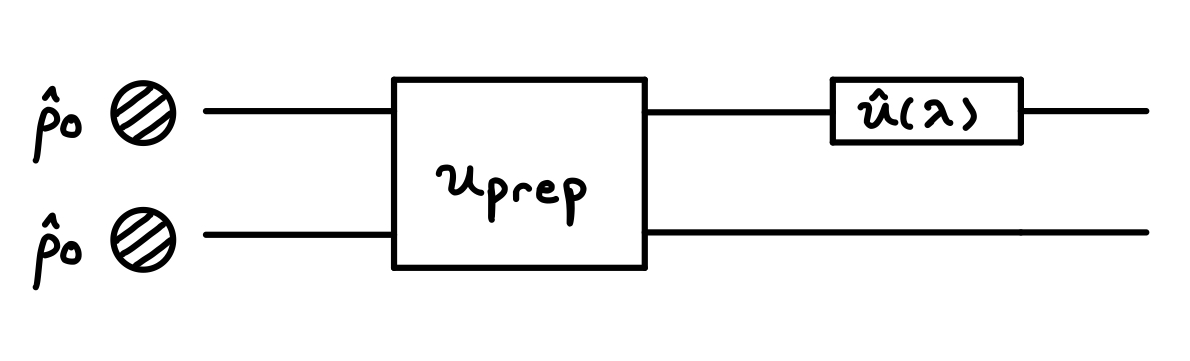
\includegraphics[width=0.90\linewidth]{Two-Particle-One-Unitary-QFI.jpg}
\caption{Schematic of two particle unitary evolution.}
\end{center}
\end{figure}
\newline
Take for instance the unitary operator operator that is constructed via $\hat{U}(\lambda)\otimes\hat{I}$ from equation (\ref{eq:29})
%--------------------------------------------------
%	Equation (83)
%--------------------------------------------------
\begin{equation} \label{eq:83}
\hat{U}(\lambda)=
\left(\begin{array}{cccc}
e^{-i\lambda/2} & 0 & 0 & 0 \\
0 & e^{-i\lambda/2} & 0 & 0 \\
0 & 0 & e^{i\lambda/2} & 0 \\
0 & 0 & 0 & e^{i\lambda/2} \\
\end{array}\right)
\end{equation}
that acts on the density operator
%--------------------------------------------------
%	Equation (84)
%--------------------------------------------------
\begin{equation} \label{eq:84}
\hat{\rho}=\frac{1}{16}
\left(\begin{array}{cccc}
4+4r^2 & 0 & 0 & -8ir \\
0 & 4-4r^2 & 0 & 0 \\
0 & 0 & 4-4r^2 & 0 \\
8ir & 0 & 0 & 4+4r^2 \\
\end{array}\right).
\end{equation}
$U_{\text{prep}}$ is the unitary of when equation (\ref{eq:83}) acts on equation (\ref{eq:84}). We can calculate the Quantum Fisher Information for a two particle system in a similar manner of the single particle system. The only difference is that there is a $4\times4$ matrix that actually consists of two $2\times2$ matrices. So we just have to calculate the Quantum Fisher Information of each matrix and then add them together. When the matrix in equation (\ref{eq:83}) acts on the matrix in (\ref{eq:84}) the Quantum Fisher Information is
%--------------------------------------------------
%	Equation (85)
%--------------------------------------------------
\begin{equation} \label{eq:85}
H=\frac{2r^2}{1+r^2}.
\end{equation}

When we compare the single particle result to the two particle result for very noisy states the two particle state has twice the Quantum Fisher Information for very noisy states. When the states are not very noisy, the advantage of this method is $2/(1+r^2)$. Once again though the two particle system is more accurate in estimating the parameter compared to that of the single particle system. 
%---------------------------------------------------------------------------
%	Modeling of Noise
%---------------------------------------------------------------------------
\section*{Modeling of Noise}
In this section we will be discussing the modeling of noise and the evolution that they have on density operators. The noise that gets implemented into these measurements will decrease the accuracy of the parameter estimation. This evolution for the specific example of rotation about the $z$ axis of $\pi$ with probability $(1-\alpha)$ and $\alpha$ can be calculated via
%--------------------------------------------------
%	Equation (86)
%--------------------------------------------------
\begin{equation} \label{eq:86}
\hat{\rho}_f=(1-\alpha)\hat{\rho}_i+\alpha\hspace{1pt}\hat{\sigma}_z\hat{\rho}_i\hat{\sigma}_z
\end{equation}
where $\alpha$ is a parameter between zero and one. This phenomenon is called a phase flip and possibly rotates the particle around the $z$ axis. For particles that are originally oriented in the $z$ and $-z$ directions there is no change in orientation. If we examine a particle originally oriented in the $+x$ direction with a density operator 
%--------------------------------------------------
%	Equation (87)
%--------------------------------------------------
\begin{equation} \label{eq:87}
\hat{\rho}=\frac{1}{2}
\begin{pmatrix}
1 & 1 \\
1 & 1
\end{pmatrix},
\end{equation}
the state after is
%--------------------------------------------------
%	Equation (88)
%--------------------------------------------------
\begin{equation} \label{eq:88}
\hat{\rho}=\frac{1}{2}
\begin{pmatrix}
1 & 1-2\alpha \\
1-2\alpha & 1
\end{pmatrix}.
\end{equation}
This operator can also be written in the form
%--------------------------------------------------
%	Equation (89)
%--------------------------------------------------
\begin{equation} \label{eq:89}
\hat{\rho}=\frac{1}{2}\big(\hat{I}+(1-2\alpha)\hat{\sigma}_x\big).
\end{equation}
If we examine another initial direction for how noise evolves a particle, say the $-y$ direction with the density operator of 
%--------------------------------------------------
%	Equation (90)
%--------------------------------------------------
\begin{equation} \label{eq:90}
\hat{\rho}=\frac{1}{2}
\begin{pmatrix}
1 & i \\
-i & 1
\end{pmatrix}
\end{equation}
originally, the state after is
%--------------------------------------------------
%	Equation (91)
%--------------------------------------------------
\begin{equation} \label{eq:91}
\hat{\rho}=\frac{1}{2}
\begin{pmatrix}
1 & i(1-2\alpha) \\
i(2\alpha-1) & 1
\end{pmatrix}.
\end{equation}
This final density operator can be written in the form of 
%--------------------------------------------------
%	Equation (92)
%--------------------------------------------------
\begin{equation} \label{eq:92}
\hat{\rho}=\frac{1}{2}\big(\hat{I}+(2\alpha-1)\hat{\sigma}_y\big).
\end{equation}
These calculations are vital for understanding how particles evolve in certain systems when we are trying to obtain measurement estimates. 

The evolution of the states that undergo this noise can be summarized as follows. The state $\ket{0}\bra{0}$ goes to $\ket{0}\bra{0}$. The same can be said for the state $\ket{1}\bra{1}$ goes to $\ket{1}\bra{1}$. The state $\ket{0}\bra{1}$ goes to $(1-2\alpha)\ket{0}\bra{1}$ and the state $\ket{1}\bra{0}$ goes to $(1-2\alpha)\ket{1}\bra{0}$. There will be different evolutions for different $\hat{\sigma}_c$'s in equation (\ref{eq:86}).
%---------------------------------------------------------------------------
%	Quantum Fisher Information Involving Phase Flips
%---------------------------------------------------------------------------
\section*{Quantum Fisher Information Involving Phase Flips}
Now that we have an understanding of how we model noise we can move on to estimating parameters in these situations where noise exist. Using the density operator in equation (\ref{eq:84}) and the unitary operator in equation (\ref{eq:83}) we wish to examine how good of an estimation procedure this is. With this scenario, one particle is being influenced by the unitary operator and the other is undergoing a phase flip defined by equation (\ref{eq:86}) in Figure 11. 
%--------------------------------------------------
%	Figure 11
%--------------------------------------------------
\begin{figure}[htpb]
\begin{center}
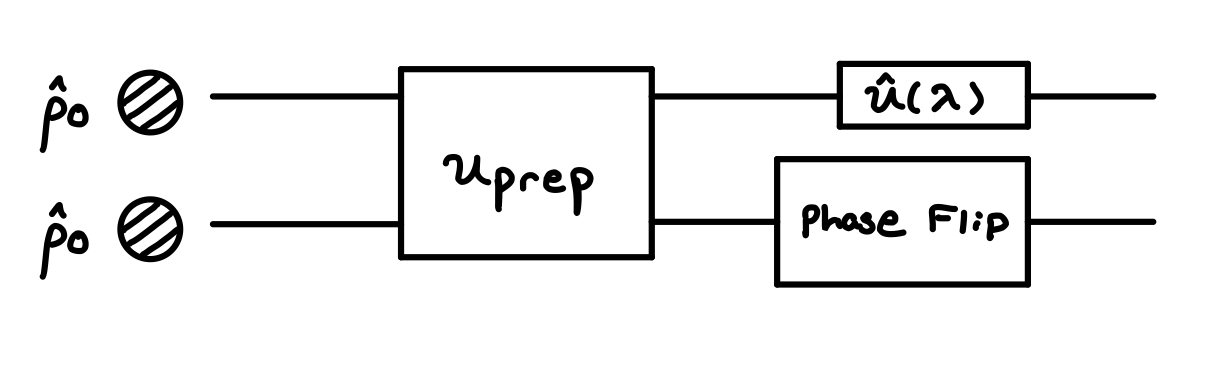
\includegraphics[width=0.90\linewidth]{Two-Particle-Phase-Flip.jpg}
\caption{Schematic of two particle one channel phase flip evolution.}
\end{center}
\end{figure}
\newline
The resulting Quantum Fisher Information is
%--------------------------------------------------
%	Equation (93)
%--------------------------------------------------
\begin{equation}\label{eq:93}
H=\frac{2r^2(1-2\alpha)^2}{(1+r^2)}.
\end{equation}
When $2(1-2\alpha)^2/(1+r^2)>1$ the result in equation (\ref{eq:93}) is a better estimation than that of equation (\ref{eq:82}).

The $\alpha$ value in equation (\ref{eq:86}) defines how noisy our state is. If $\alpha=0$ then the state is not noisy at all and it is pure. If $\alpha=1$ then the state is very noisy. When we examine the extremes of this scenario, i.e $\alpha=0$ or $\alpha=1$ we have the Quantum Fisher Information in equation (\ref{eq:85}). When $\alpha=1/2$ the Quantum Fisher Information is 0 and the parameter cannot be estimated.

We can examine the same scenario but instead of $\hat{\sigma}_z$ in equation (\ref{eq:80}) we will examine a bit flip with $\hat{\sigma}_x$. When this scenario is examined and the calculation is done, the Quantum Fisher Information is
%--------------------------------------------------
%	Equation (94)
%--------------------------------------------------
\begin{equation}\label{eq:94}
H=\frac{2r^2\alpha^2}{((2\alpha-1)r^2+1)}+\frac{2r^2(1-\alpha)^2}{(1-(2\alpha-1)r^2)}.
\end{equation}
When we examine the same extreme scenarios we still get the result in equation (\ref{eq:85}).
%---------------------------------------------------------------------------
%	Additional Phase Flips
%---------------------------------------------------------------------------
\section*{Additional Phase Flips}
Now that phase flips have been examined, measurements can be taken of previous scenarios that now involve a phase flip. Take for instance the measurement that resulted in having a the Quantum Fisher Information come out to be $H=r^2$ represented by the result found in equation (\ref{eq:82}). Taking the previous scenario and adding a phase flip can be represented by the following schematic in Figure 12.
%--------------------------------------------------
%	Figure 12
%--------------------------------------------------
\begin{figure}[h]
\begin{center}
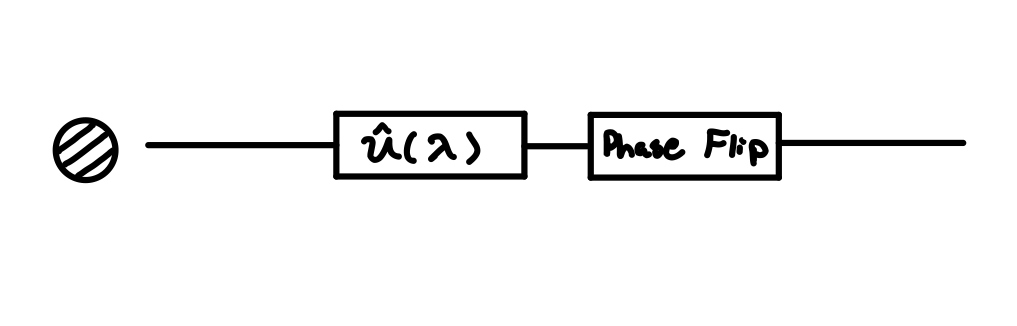
\includegraphics[width=0.70\linewidth]{SP-Phase-Flip.PNG}
\caption{Single particle measurement with a phase flip.}
\end{center}
\end{figure}
\newline
The measurement that is depicted in Figure 12 involves one particle with the unitary $\hat{U}(\lambda)=e^{-i\hat{\sigma}_z\lambda/2}$ and a phase flip in the $z$ direction. When this is calculated the Quantum Fisher Information comes out to be
%--------------------------------------------------
%	Equation (95)
%--------------------------------------------------
\begin{equation}\label{eq:95}
H=r^2(1-2\alpha)^2
\end{equation}
where $\alpha$ comes from the phase flip in Figure 12. The difference between this result as seen in equation (\ref{eq:95}) and the result in equation (\ref{eq:82}) is the $1-2\alpha$ component. This is coming from the phase flip that the spin - 1/2 particle experiences. Without this phase flip, the measurement is more precise. With the phase flip introduced the measurement of the parameter at question is subsequent to be interfered with and thus is less accurate.

This process of introducing a phase flip to previous measurements can also be implemented to the result in equation (\ref{eq:93}). This measurement had one particle undergo a phase flip while the other particle evolved under a unitary operator. Now, in this new scenario the particle that evolved under a unitary operator will also undergo a phase flip as well. Schematically this can be represented by the diagram shown in Figure 13.
%--------------------------------------------------
%	Figure 13
%--------------------------------------------------
\begin{figure}[h]
\begin{center}
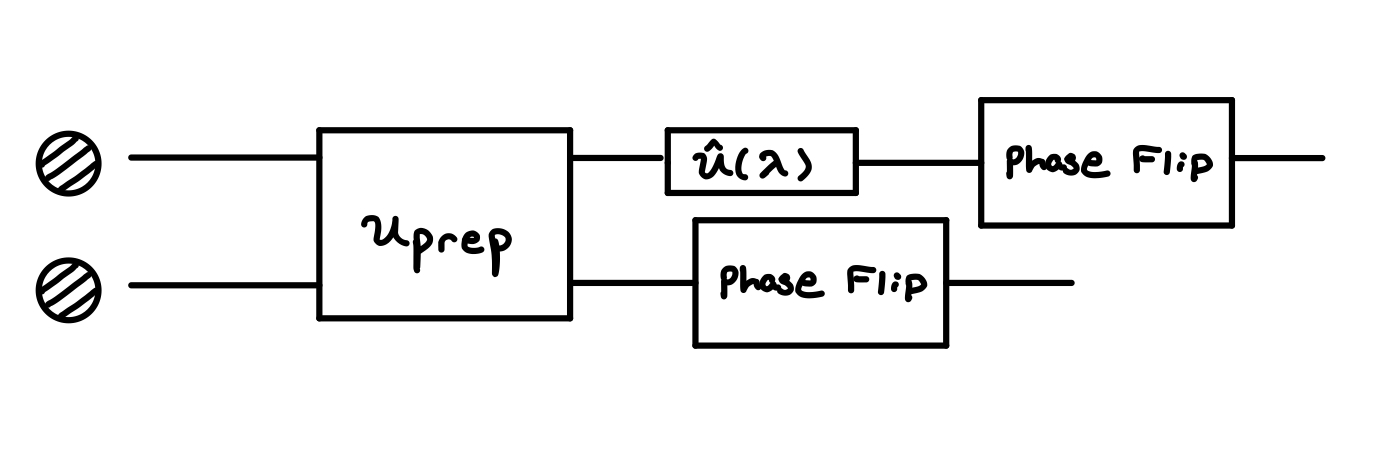
\includegraphics[width=0.70\linewidth]{TP-Dual-Phase-Flip.PNG}
\caption{Dual particle phase flip evolution. The first particle undergoes an evolution with a unitary operator and then a phase flip. The second particle undergoes only a phase flip.}
\end{center}
\end{figure}
\newpage
These particles in Figure 13 evolve under the same $U_{\text{Prep}}$ operator as those in the previous two particle scenarios. The Quantum Fisher Information is
%--------------------------------------------------
%	Equation (96)
%--------------------------------------------------
\begin{equation}\label{eq:96}
H=\frac{2r^2(1-2\alpha)^2(1-2\beta)^2}{(1+r^2)}.
\end{equation}
The $\alpha$ in equation (\ref{eq:96}) represents the top particle's phase flip in Figure 13 and the $\beta$ is the lower particle phase flip. Regardless of the extra particle undergoing a phase flip in Figure 13, this method of estimating a parameter is still more accurate than that of Figure 12. When the state of the particle is undergoing a lot of noise ($r<<1$) there is an advantage of $H=2(1-2\beta)^2$. When $\beta=1$ or $\beta=0$ there is a two-fold advantage of using the method of parameter estimation in Figure 13 compared to that of the method in Figure 12.
%---------------------------------------------------------------------------
%	Depolarizing Channels
%---------------------------------------------------------------------------
\section*{Depolarizing Channels}
The topic of depolarizing channels will now be discussed. This measurement can be represented schematically as seen in Figure 14.
%--------------------------------------------------
%	Figure 14
%--------------------------------------------------
\begin{figure}[h]
\begin{center}
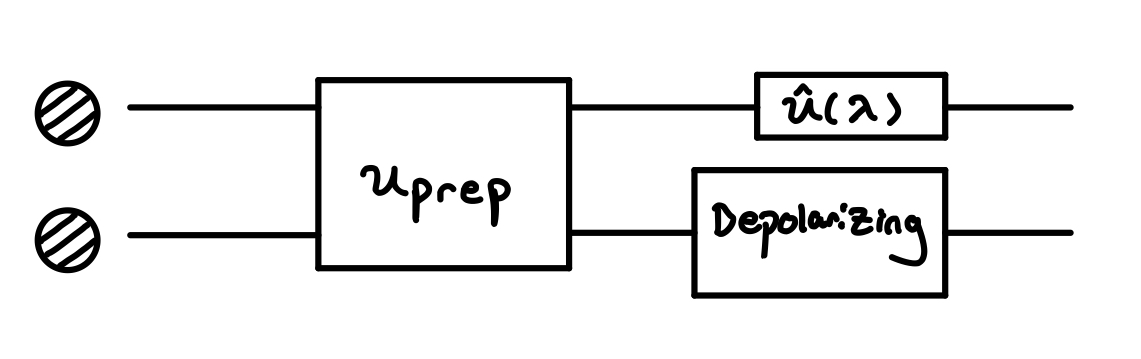
\includegraphics[width=0.66\linewidth]{TP-Depolarizing.PNG}
\caption{Two particle system with one particle undergoing a unitary evolution and the other a depolarization.}
\end{center}
\end{figure}
\newline
The way these particles undergo a depolarization can be calculated via
%--------------------------------------------------
%	Equation (97)
%--------------------------------------------------
\begin{equation}\label{eq:97}
\hat{\rho}_f=\Big(\frac{1-\alpha}{2}\Big)\text{Tr}[\hat{\rho}_i]\hat{I}+\alpha\hat{\rho}_i
\end{equation}
where the $\hat{\rho}$ in equation (\ref{eq:97}) represents the particle that is undergoing a depolarization. When this scenario in Figure 14 is calculated, the Quantum Fisher Information comes out to be
%--------------------------------------------------
%	Equation (98)
%--------------------------------------------------
\begin{equation}\label{eq:98}
H=\frac{4r^2\alpha^2}{(1+r^2)(1+\alpha)+(1-r^2)(1-\alpha)}.
\end{equation}
When the result in equation (\ref{eq:98}) is compared to that of the scenario in Figure 12 along with the states ($r<<1$) the Quantum Fisher Information is then $H=2\alpha^2$. When $\alpha=1$ (Polarization is minimal) this method has a two-fold advantage when estimating the parameter.
%---------------------------------------------------------------------------
%	Phase Flip With Lambda Parameter
%---------------------------------------------------------------------------
\section*{Phase Flip With $\lambda$ Parameter}
Previously phase flips with $\alpha$ as the parameter have been discussed. Now phase flips with a $\lambda$ as the parameter will be discussed. We are pursuing to estimate the parameter $\lambda$ and this phase flip is calculated via
%--------------------------------------------------
%	Equation (99)
%--------------------------------------------------
\begin{equation}\label{eq:99}
\hat{\rho}_f=(1-\lambda)\hat{\rho}_i+\lambda\hspace{1pt}\hat{\sigma}_z\hat{\rho}_i\hat{\sigma}_z
\end{equation}
where equation (\ref{eq:99}) is the same as equation (\ref{eq:86}) but with a $\lambda$ instead of an $\alpha$. One can perform this calculation for one or multiple particles and then calculate the Quantum Fisher Information. The first scenario that will be examined is a single particle undergoing this phase flip evolution and then calculating the Quantum Fisher Information after. This scenario can be seen in Figure 15.
%--------------------------------------------------
%	Figure 15
%--------------------------------------------------
\begin{figure}[h]
\begin{center}
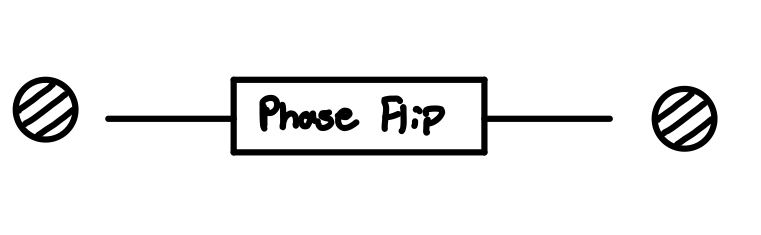
\includegraphics[width=0.65\linewidth]{Single-Particle-Phase-Flip-Evolution-Schematic.jpg}
\caption{A single particle evolution through the phase flip defined in Equation (\ref{eq:99}). After this particle undergoes the phase flip the QFI is calculated.}
\end{center}
\end{figure}
\newline
The Quantum Fisher Information for the scenario in Figure 15 is
%--------------------------------------------------
%	Equation (100)
%--------------------------------------------------
\begin{equation}\label{eq:100}
H=\frac{4r^2}{1-r^2(1-2\lambda)^2}.
\end{equation}
One can now ask questions about what the Quantum Fisher Information of this measurement becomes with $\lambda$ values $<<$ 1 and $r$ values $<<$ 1. How the Quantum Fisher Information of this measurement changes with varying $\lambda$ and $r$ values can be seen in Figure 16.
\newline
%--------------------------------------------------
%	Figure 16
%--------------------------------------------------
\begin{figure}[h]
\begin{center}
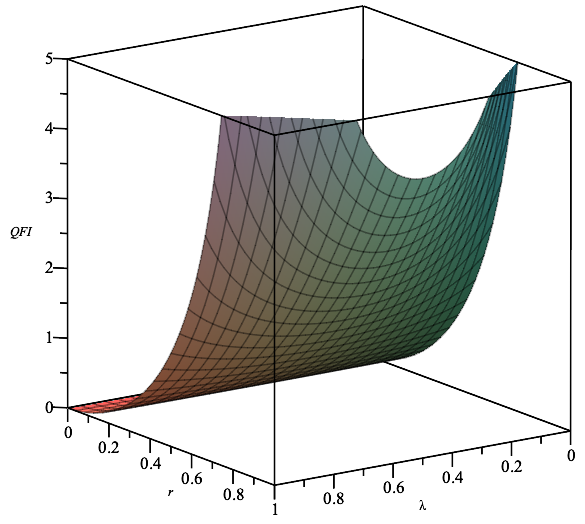
\includegraphics[width=0.65\linewidth]{Phase-Flip-Lambda-QFI-Graph.png}
\caption{Quantum Fisher Information of the scenario depicted in Figure 15.}
\end{center}
\end{figure}
\newline
As the initial state of the system becomes more noisy the Quantum Fisher Information of this calculation approaches $0$. The $\lambda$ value in Equation (\ref{eq:100}) is less influential to the overall Quantum Fisher Information compared to that of the $r$ value. A dual particle evolution can now be looked at.

We are now interested in examining a scenario where two particles enter a unitary operator and one particle is then subjected to a phase flip with the parameter $\lambda$. This unitary operator labeled $\hat{U}_{prep}$ is a unitary matrix that consists of single qubit interactions where one of these interactions is between two particles. The first channel of the measurement is subjected to a phase flip and the second channel is left undisturbed. This second channel is sometimes referred to as the spectator of the measurement. This can be seen in Figure 17.
%--------------------------------------------------
%	Figure 17
%--------------------------------------------------
\begin{figure}[h]
\begin{center}
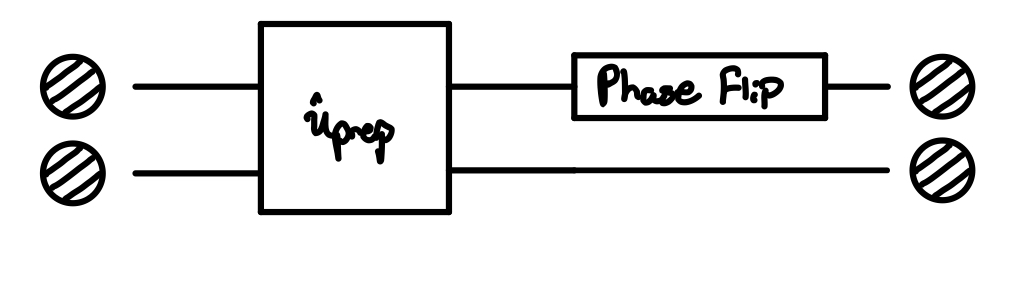
\includegraphics[width=0.65\linewidth]{Two-Particle-Phase-Flip-Single-Channel-Lambda-Schematic.jpeg}
\caption{Two particles enter the $\hat{U}_{\text{prep}}$ unitary operator and then the first particle is subjected to a phase flip defined by Equation (\ref{eq:99}).}
\end{center}
\end{figure}
\newline
When the Quantum Fisher Information in Figure 17 is calculated it is found to be
%--------------------------------------------------
%	Equation (101)
%--------------------------------------------------
\begin{equation}\label{eq:101}
H=\frac{8r^2(1+r^2)}{(1+r^2)^2-4r^2(1-2\lambda)^2}.
\end{equation}
We can now examine when equation (\ref{eq:101}) is more advantageous to use as a measurement scheme than that of equation (\ref{eq:100}). This is done by dividing the equation (\ref{eq:101}) by that of equation (\ref{eq:100}). This result is called the gain for the protocol in Figure 17 and the gain is
%--------------------------------------------------
%	Equation (102)
%--------------------------------------------------
\begin{equation}\label{eq:102}
G=\frac{2(1+r^2)(1-r^2(1-2\lambda)^2)}{(1+r^2)^2-4r^2(1-2\lambda)^2}.
\end{equation}
Equation (\ref{eq:102}) quantifies when the scenario in Figure 17 is more advantageous than the one depicted in Figure 16. Graphically this gain can be seen in Figure 18.
%--------------------------------------------------
%	Figure 18
%--------------------------------------------------
\begin{figure}[h]
\begin{center}
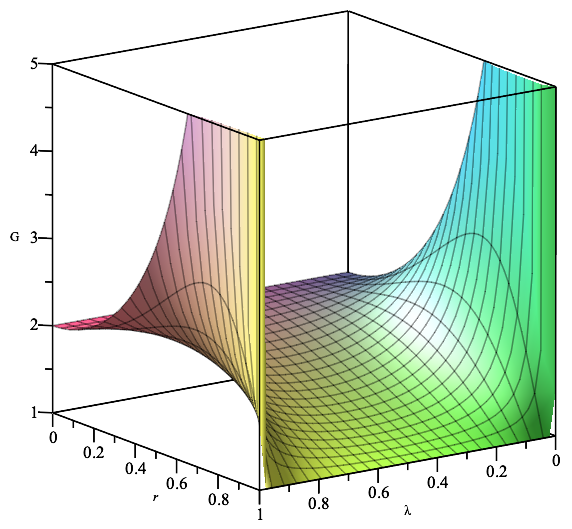
\includegraphics[width=0.65\linewidth]{Phase-Flip-One-Channel-Lambda-and-r-Gain.png}
\caption{The gain that is observed is greatest when $\lambda=0$ or $\lambda=1$ and when $r=1$.}
\end{center}
\end{figure}
\newline
There is little to no advantage using the method of measurement in Figure 17 compared to that in Figure 15 when $\lambda$ ranges between $0$ and $1$ when the original state of the system is pure. The phase flip parameter $\lambda$ becomes less and less important to the gain of the measurement when the purity of the system decreases.

We now wish to examine a scenario where both particles undergo a phase flip. The first particle undergoes a phase flip with the parameter $\lambda$ and the second undergoes a phase flip with the parameter $\alpha$. This scenario can be seen in Figure 19.
%--------------------------------------------------
%	Figure 19
%--------------------------------------------------
\begin{figure}[h]
\begin{center}
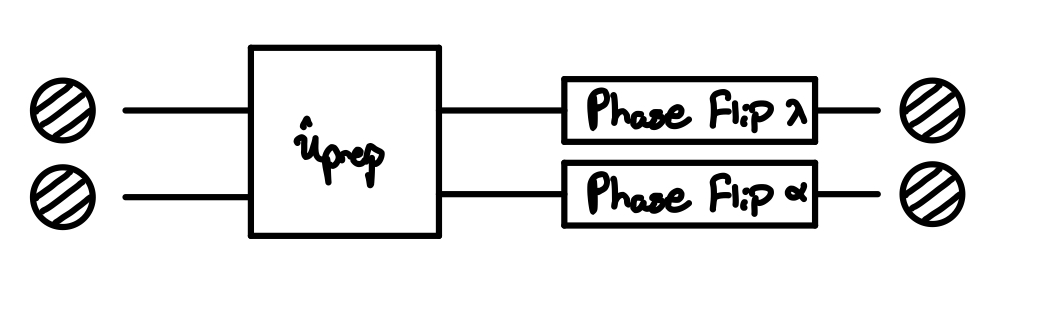
\includegraphics[width=0.65\linewidth]{Two-Particle-Phase-Flip-Dual-Channel-Alpha-Lambda-Schematic.jpg}
\caption{The first particles phase flip is characterized by $\lambda$ and the second particles phase flip is characterized by $\alpha$.}
\end{center}
\end{figure}
\newline
When the Quantum Fisher Information for this scenario is calculated it comes out to be
%--------------------------------------------------
%	Equation (103)
%--------------------------------------------------
\begin{equation}\label{eq:103}
H=\frac{8r^2(1-2\alpha)^2(1+r^2)}{(1+r^2)^2-4r^2(1-2\lambda)^2(1-2\alpha)^2}.
\end{equation}
We can now look for when the scenario in Figure 19 is more advantageous as a measuring scheme than that of Figure 15. The gain of the scenario in Figure 19 compared to the scenario in Figure 15 is
%--------------------------------------------------
%	Equation (104)
%--------------------------------------------------
\begin{equation}\label{eq:104}
G=\frac{2(1-2\alpha)^2(1+r^2)(1-r^2(1-2\lambda)^2)}{(1+r^2)^2-4r^2(1-2\lambda)^2(1-2\alpha)^2}.
\end{equation}
When $\alpha=0$ in equation (\ref{eq:104}) the gain reduces to the gain found in equation (\ref{eq:102}). Since this gain involves three variables in it, we have to choose one variable that will be held constant while the other two are varied. Since the main difference between the scenario in Figure 17 and the one in Figure 19 is the additional phase flip $\alpha$ we will choose to hold $\alpha$ constant. When $\alpha=0.01$ the gain of the scenario in Figure 19 compared to that of Figure 15 can be seen in Figure 20.
\newpage
%--------------------------------------------------
%	Figure 20
%--------------------------------------------------
\begin{figure}[h]
\begin{center}
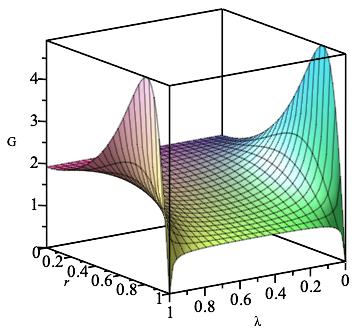
\includegraphics[width=0.65\linewidth]{Phase-Flip-Two-Channel-Alpha=001-Gain.png}
\caption{Gain when $\alpha=0.01$.}
\end{center}
\end{figure}
This gain is when $\alpha<<1$ and almost doesn't contribute to the Quantum Fisher Information. We can now increase the value of $\alpha$ to $0.1$ and graph it again. This result can be seen in Figure 21.
%--------------------------------------------------
%	Figure 21
%--------------------------------------------------
\begin{figure}[h]
\begin{center}
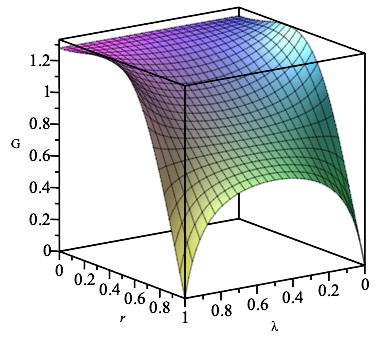
\includegraphics[width=0.65\linewidth]{Phase-Flip-Two-Channel-Alpha=01-Gain.png}
\caption{Gain when $\alpha=0.1$.}
\end{center}
\end{figure}
\newline
When the $\alpha$ valued is increased to $0.1$ from $0.01$ the gain is decreased. This shows that the second phase flip is being destructive to our measurements and in turn is proving to not be as beneficial. There is still some gain when $r\approx0.5$ is lower or higher but it isn't anything that is extremely greater. Changing $\alpha$ to $0.2$ from $0.1$ Figure 22 is produced.
\newpage
%--------------------------------------------------
%	Figure 22
%--------------------------------------------------
\begin{figure}[h]
\begin{center}
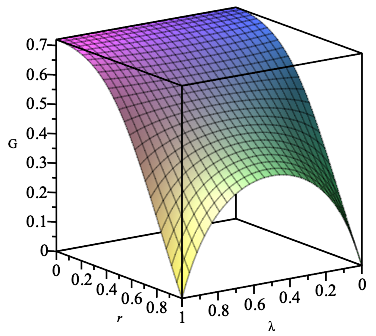
\includegraphics[width=0.65\linewidth]{Phase-Flip-Two-Channel-Alpha=02-Gain.png}
\caption{Gain when $\alpha=0.2$.}
\end{center}
\end{figure}
When $\alpha=0.2$ the scenario in Figure 19 is not beneficial to the scenario in Figure 15. In fact Figure 19 proves to be detrimental to that of Figure 15. This detriment is just exacerbated when the value of $\alpha$ increases and we can observe this when $\alpha=0.3$ in Figure 19.
%--------------------------------------------------
%	Figure 23
%--------------------------------------------------
\begin{figure}[h]
\begin{center}
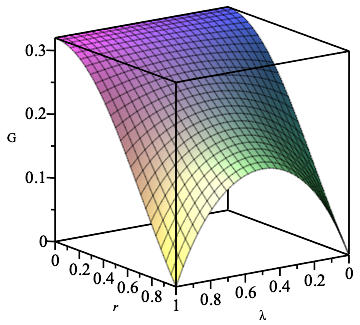
\includegraphics[width=0.65\linewidth]{Phase-Flip-Two-Channel-Alpha=03-Gain.png}
\caption{Gain when $\alpha=0.3$.}
\end{center}
\end{figure}
\newline
At this point the gain when $\alpha=0.3$ is almost a third at the best point that is possible. We would be better off using the scenario in Figure 15 as a measurement procedure compared to that of the one found in Figure 19. The gain is decreased even more when $\alpha=0.4$ and can be seen in Figure 24.
\newpage
%--------------------------------------------------
%	Figure 24
%--------------------------------------------------
\begin{figure}[h]
\begin{center}
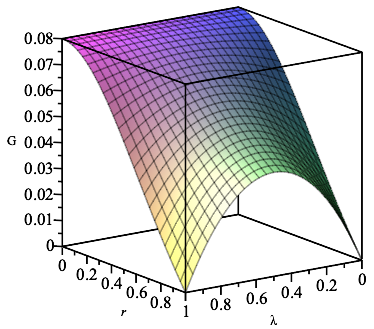
\includegraphics[width=0.65\linewidth]{Phase-Flip-Two-Channel-Alpha=04-Gain.png}
\caption{Gain when $\alpha=0.4$.}
\end{center}
\end{figure}
The Quantum Fisher Information and gain is decreased to zero when $\alpha=0.5$ and this can be seen in Figure 25.
%--------------------------------------------------
%	Figure 25
%--------------------------------------------------
\begin{figure}[h]
\begin{center}
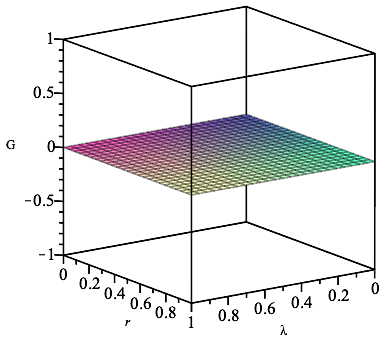
\includegraphics[width=0.65\linewidth]{Phase-Flip-Two-Channel-Alpha=05-Gain.png}
\caption{Gain when $\alpha=0.5$.}
\end{center}
\end{figure}
\newline
At certain choices of $\alpha$ it is not advantageous to use the method depicted in Figure 19 compared to that of Figure 15. For very specific values of $\alpha$ it is disastrous to use the method in Figure 19 compared to that in Figure 15. This happens when $\alpha=0.5$. 

An inequality can be determined to describe when using the scenario in Figure 19 is advantageous to that of the scenario in Figure 15. This inequality is
%--------------------------------------------------
%	Equation (105)
%--------------------------------------------------
\begin{equation}\label{eq:105}
\alpha < \frac{1}{2}\Bigg(1-\sqrt{\frac{\gamma^2}{2\gamma-2r^2\eta^2\gamma+4r^2\eta^2}}\Bigg)
\end{equation}
where $\gamma=(1+r^2)$ and $\eta=(1-2\lambda)$. Equation (\ref{eq:105}) shows that for only certain values of $\alpha$ the scenario in Figure 19 is more useful as a measuring tactic compared to that of Figure 15. What this inequality ends up showing is that for noisy states Figure 19 is more useful than that of Figure 15. Graphically this inequality can be seen in Figure 26.
%--------------------------------------------------
%	Figure 26
%--------------------------------------------------
\begin{figure}[h]
\begin{center}
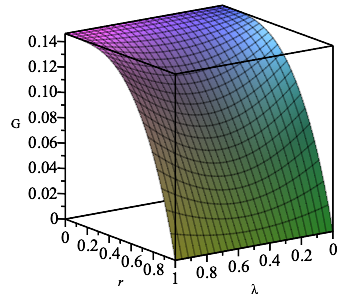
\includegraphics[width=0.65\linewidth]{Phase-Flip-Alpha-Inequality-Graph.png}
\caption{Graph of the inequality in Equation (\ref{eq:105}). This graph tells what $\alpha$ will limit the gain. As the initial state becomes more pure the advantage of the scenario in Figure 19 becomes less advantageous than that of Figure 15.}
\end{center}
\end{figure}
\newline
The gain in Figure 26 decreases significantly as the initial state becomes more pure. What can be taken away from this is that for certain values of $\alpha$ it is more advantageous to use the scenario in Figure 15 than that of the scenario in Figure 19. This same analysis can be conducted for the depolarizing channels and measurements that use multiple depolarizing channels.
%---------------------------------------------------------------------------
%	Multiple Depolarizing Channels
%---------------------------------------------------------------------------
\section*{Multiple Depolarizing Channels}
Phase flips with multiple parameters have been covered and the same will now be done for depolarizing channels. We will first examine the scenario of a single particle undergoing a depolarizing evolution. Schematically this can be seen in Figure 27.
\newpage
%--------------------------------------------------
%	Figure 27
%--------------------------------------------------
\begin{figure}[h]
\begin{center}
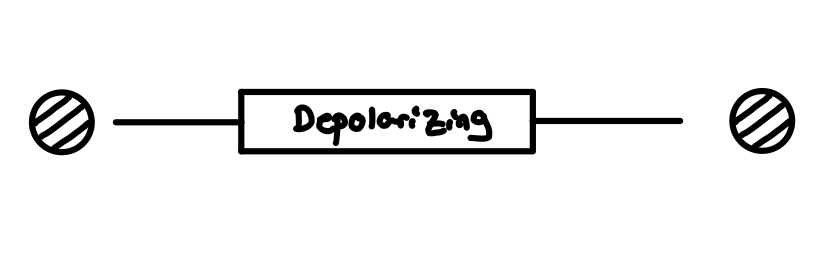
\includegraphics[width=0.65\linewidth]{Depolarizing-Single-Channel-Lambda-Schematic.jpg}
\caption{Schematic of a single particle depolarizing channel evolution.}
\end{center}
\end{figure}
When the calculation is done the Quantum Fisher Information of Figure 27 is
%--------------------------------------------------
%	Equation (106)
%--------------------------------------------------
\begin{equation}\label{eq:106}
H=\frac{r^2}{1-r^2\lambda^2}.
\end{equation}
Graphically the Quantum Fisher Information of Figure 27 can be seen in Figure 28.
%--------------------------------------------------
%	Figure 28
%--------------------------------------------------
\begin{figure}[h]
\begin{center}
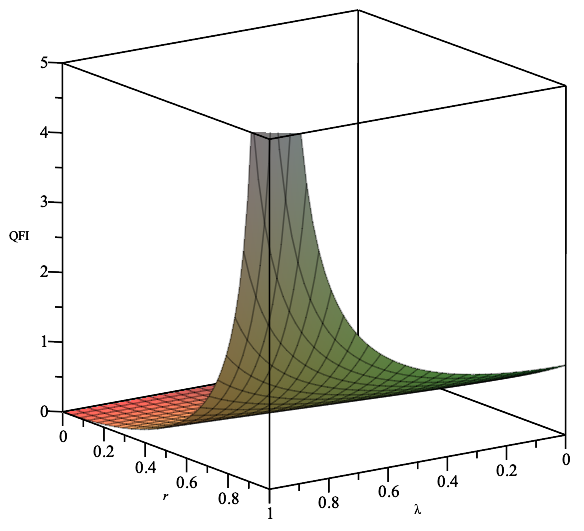
\includegraphics[width=0.65\linewidth]{Depolarizing-Single-Channel-QFI.png}
\caption{Quantum Fisher Information of a single particle depolarizing channel evolution.}
\end{center}
\end{figure}
\newline
As the initial state of the particle becomes less noisy and the $\lambda$ value approaches 1, the Quantum Fisher Information of the scenario in Figure 27 explodes towards infinity. We wish to examine situations in which there are two particles and depolarizing channels are being used.

The first scenario with multiple particles and depolarizing channels that will be examined can be seen in the schematic of Figure 29.
\newpage
%--------------------------------------------------
%	Figure 29
%--------------------------------------------------
\begin{figure}[h]
\begin{center}
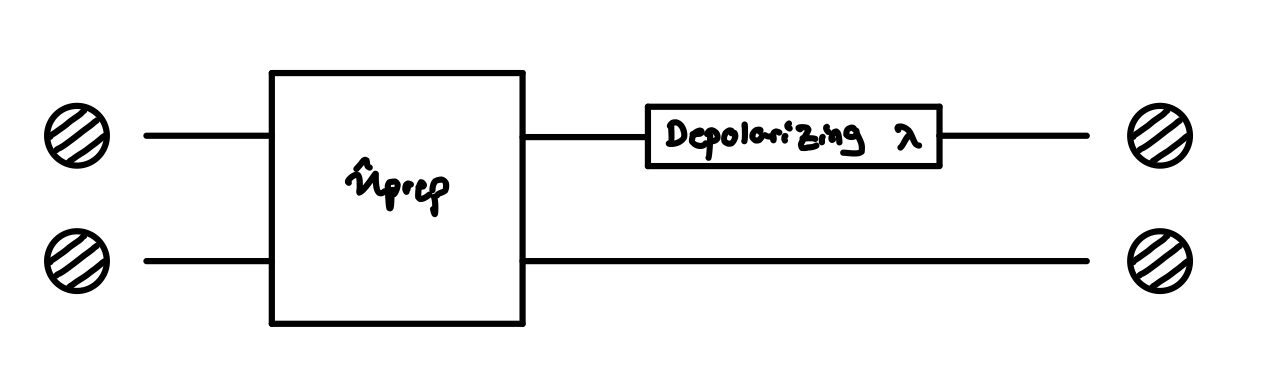
\includegraphics[width=0.65\linewidth]{Depolarizing-Double-Channel-Lambda-Schematic.jpg}
\caption{Schematic of two particle measurement where one particle undergoes a depolarizing evolution with parameter $\lambda$.}
\end{center}
\end{figure}
When the Quantum Fisher Information is calculated for this scenario it comes out to be
%--------------------------------------------------
%	Equation (107)
%--------------------------------------------------
\begin{equation}\label{eq:107}
H=\frac{r^2(r^2(1-4\lambda)+r^4\lambda+2)}{(1+2r\lambda+r^2\lambda)(1-2r\lambda+r^2\lambda)(1-r^2\lambda)}.
\end{equation}
When comparing the result of the Quantum Fisher Information in equation (\ref{eq:107}) to the result in equation (\ref{eq:106}), the gain of the scenario in Figure 29 over Figure 27 is
%--------------------------------------------------
%	Equation (108)
%--------------------------------------------------
\begin{equation}\label{eq:108}
G=\frac{(r^2\lambda^2-1)(r^4\lambda-4r^2\lambda+r^2+2)}{(1+2r\lambda+r^2\lambda)(1-2r\lambda+r^2\lambda)(r^2\lambda-1)}.
\end{equation}
We can graph this gain and it can be seen in Figure 30.
%--------------------------------------------------
%	Figure 30
%--------------------------------------------------
\begin{figure}[h]
\begin{center}
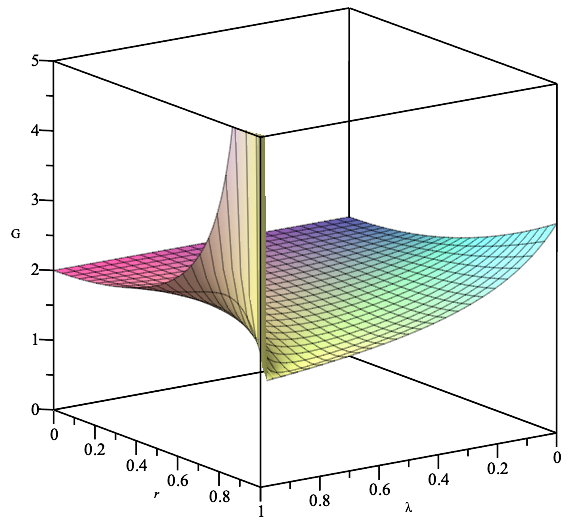
\includegraphics[width=0.65\linewidth]{Depolarizing-Double-Channel-Lambda-Gain-Graph.png}
\caption{Graph of the gain for the scenario in Figure 29 over Figure 27.}
\end{center}
\end{figure}
\newline
When the scenario in Figure 29 is conducted it is always advantageous over the scenario in Figure 27. There are no values for $r$ and $\lambda$ where the single channel is advantageous to that over the double channel.

In this last scenario two particles undergo depolarization, one with parameter $\lambda$ and the other $\alpha$. The schematic of this measurement can be seen in Figure 31.
%--------------------------------------------------
%	Figure 31
%--------------------------------------------------
\begin{figure}[h]
\begin{center}
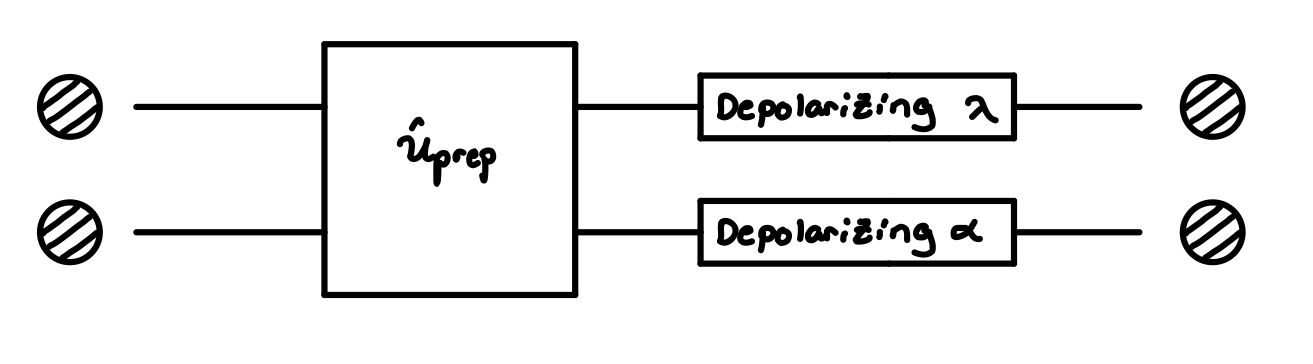
\includegraphics[width=0.65\linewidth]{Depolarizing-Double-Channel-Alpha-and-Lambda-Schematic.jpg}
\caption{Schematic of two particle measurement where the first particle undergoes a depolarizing evolution with parameter $\lambda$ and the second particle undergoes a depolarizing evolution with parameter $\alpha$.}
\end{center}
\end{figure}
\newline
The Quantum Fisher Information of the scenario in Figure 31 comes out to be
%--------------------------------------------------
%	Equation (109)
%--------------------------------------------------
\begin{equation}\label{eq:109}
H=\frac{r^2\alpha^2(\alpha\lambda r^4-4r^2\lambda\alpha+r^2+2)}{(1-r^2\lambda\alpha)(1+r\alpha(r+2)\lambda)(1+r\alpha(r-2)\lambda)}.
\end{equation}
The gain equation for Figure 31 over Figure 27 comes out to be
%--------------------------------------------------
%	Equation (110)
%--------------------------------------------------
\begin{equation}\label{eq:110}
G=\frac{\alpha^2(\alpha\lambda r^4-4\lambda r^2\alpha+r^2+2)^2(r^2\lambda^2-1)}{(\lambda r^2\alpha-1)(1+r\alpha(r+2)\lambda)(1+r\alpha(r-2)\lambda)}.
\end{equation}
The gain of Figure 31 over that of Figure 27 with $r=0.01$ can be seen in Figure 32.
%--------------------------------------------------
%	Figure 32
%--------------------------------------------------
\begin{figure}[h]
\begin{center}
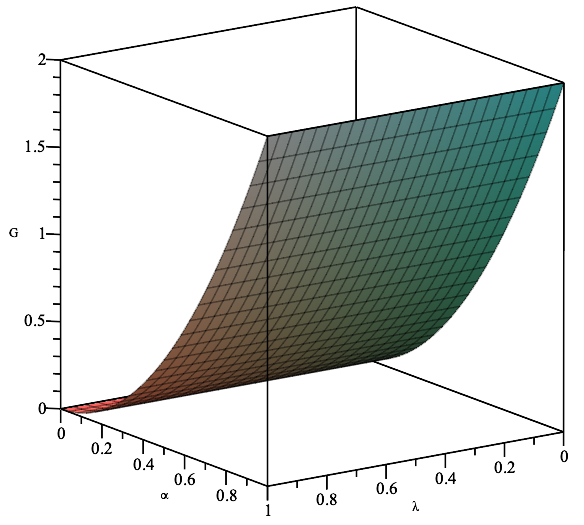
\includegraphics[width=0.65\linewidth]{Depolarizing-Double-Channel-Alpha-and-Lambda-r=001-Gain-Graph.png}
\caption{Gain of Figure 31 over Figure 27 with $r=0.01$.}
\end{center}
\end{figure}
\newline
In this instance there is some gain for specific values of $\alpha$ and $\lambda$ for initial noisy states. The next scenario to examine is when the initial states are pure (i.e $r=1.0$). The gain of Figure 31 over that of Figure 27 with pure initial states can be seen in Figure 33.
%--------------------------------------------------
%	Figure 33
%--------------------------------------------------
\begin{figure}[h]
\begin{center}
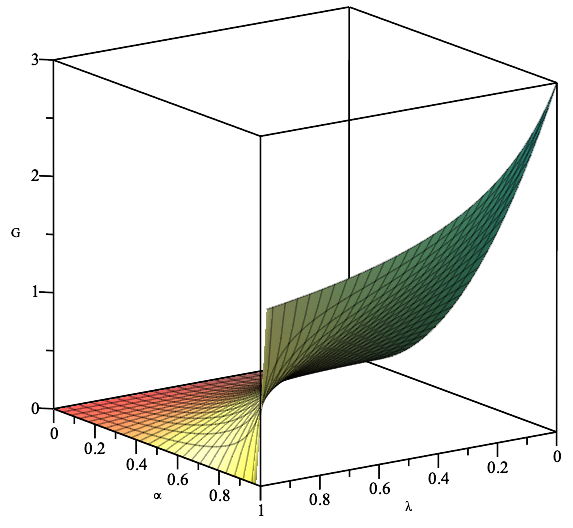
\includegraphics[width=0.65\linewidth]{Depolarizing-Double-Channel-Alpha-and-Lambda-r=1-Gain-Graph.png}
\caption{Gain of Figure 31 over Figure 27 with $r=1.0$.}
\end{center}
\end{figure}
\newline
The result of Figure 33 tells us that there are specific values of $\alpha$ and $\lambda$ that will produce a positive gain for that of Figure 31 over Figure 27. Otherwise it is advantageous to use the scenario in Figure 27.
%---------------------------------------------------------------------------
%	Three Particle Phase Flip
%---------------------------------------------------------------------------
\section*{Three Particle Phase Flip}
We now move on to investigating phase flips with three particles. The measurement that is being investigated can be seen in Figure 34.
%--------------------------------------------------
%	Figure 34
%--------------------------------------------------
\begin{figure}[h]
\begin{center}
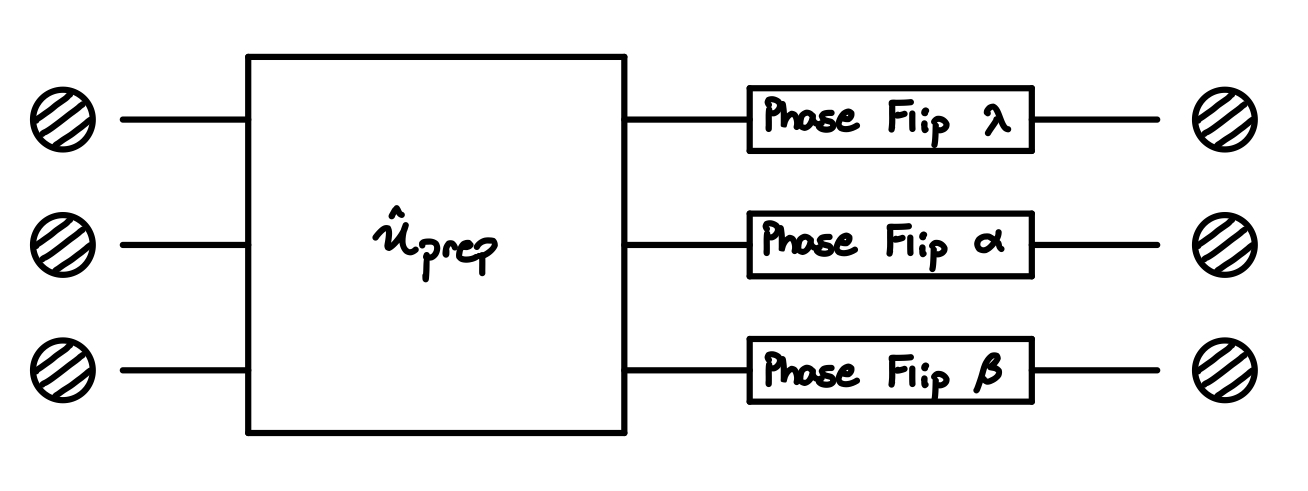
\includegraphics[width=0.65\linewidth]{Phase-Flip-Triple-Channel-Lambda-Schematic.jpg}
\caption{Phase flip measurement with a three particle system.}
\end{center}
\end{figure}
\newline
Figure 34 depicts a measurement where three particles are subjected to a phase flip. Each phase flip is represented by its own parameter where the parameter that we are trying to estimate is $\lambda$. With this, the Quantum Fisher Information comes out to be
%--------------------------------------------------
%	Equation (111)
%--------------------------------------------------
\begin{align}\label{eq:111}
H&=r^2(1-2\alpha)^2(1-2\beta)^2\cdot \nonumber \\
\bigg(&\frac{(r+3)^2(3r^2+1)(\eta)+3(1-r^2)^3(\xi)}{(\eta)(\xi)}\bigg)
\end{align}
where $\eta=(1-r^2)^2-\gamma^2r^2(1-r^2)^2$, $\xi=(3r^2+1)^2-r^2(r+3)^2\gamma^2$, and $\gamma=(1-2\lambda)(1-2\alpha)(1-2\beta)$. We can continue to find the gain of the scenario in Figure 34 over that of Figure 15 with parameter lambda. The gain equation is thus
%--------------------------------------------------
%	Equation (112)
%--------------------------------------------------
\begin{align}\label{eq:112}
G&=\frac{1-r^2(1-2\lambda)^2(1-2\alpha)^2(1-2\beta)^2}{4}\cdot \nonumber \\
\bigg(&\frac{(r+3)^2(3r^2+1)(\eta)+3(1-r^2)^3(\xi)}{(\eta)(\xi)}\bigg).
\end{align}
Because equation (\ref{eq:112}) has four variables in it we have to limit two variables at a time when we observe the gains of this scenario. The first scenario is when the initial state is noisy ($r=0.01$) and the $\alpha$ parameter is almost nonexistent $\alpha=0.01$. The gain of this scenario can be seen in Figure 35.
%--------------------------------------------------
%	Figure 35
%--------------------------------------------------
\begin{figure}[h]
\begin{center}
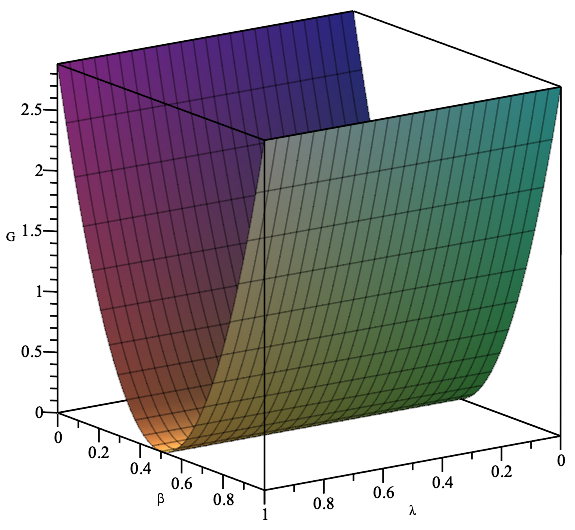
\includegraphics[width=0.65\linewidth]{Phase-Flip-Triple-Channel-r=001-Alpha=001-Gain-Graph.png}
\caption{Gain of Figure 34 over Figure 15 with $r=0.01$ and $\alpha=0.01$.}
\end{center}
\end{figure}
\newline
It can be observed that Figure 35 indicates that the value of $\lambda$ is insignificant when calculating a gain. When $\beta=0.5$ the gain in equation (\ref{eq:112}) is zero. The gain is symmetric for values of $\beta$ as $\beta$ approaches zero or one. This indicates that for specific values of $\beta$ there is a gain for Figure 34 over Figure 15, and this can be seen visually in Figure 35.

We now move on to examining the gain when $r=0.01$ and $\beta=0.01$. The gain for when the initial states are noisy and $\beta$ is almost nonexistent can be seen in Figure 36.
%--------------------------------------------------
%	Figure 36
%--------------------------------------------------
\begin{figure}[h]
\begin{center}
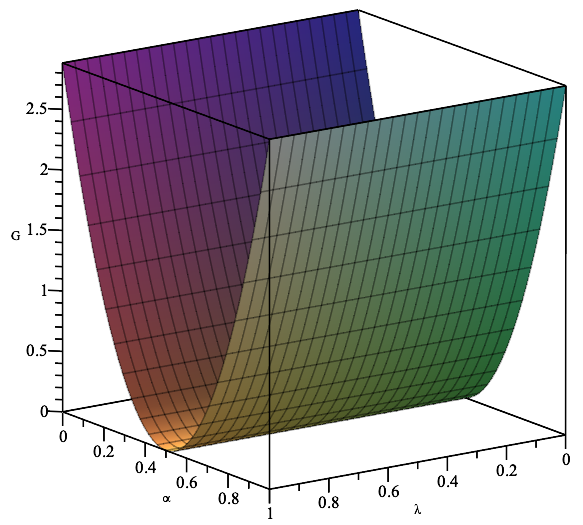
\includegraphics[width=0.65\linewidth]{Phase-Flip-Triple-Channel-r=001-Beta=001-Gain-Graph.png}
\caption{Gain of Figure 34 over Figure 15 with $r=0.01$ and $\beta=0.01$.}
\end{center}
\end{figure}
\newline
For this scenario the gain is zero when $\alpha=0.5$ and is once again symmetric as $\alpha$ approaches one or zero. This graph once again shows that there is a gain for Figure 34 over Figure 15 for specific values of $\alpha$.

The last scenario for the three particle phase flip that will be examined is when $\alpha=0.01$ and $\beta=0.01$. With this, the gain for this scenario can be seen in Figure 37.
%--------------------------------------------------
%	Figure 37
%--------------------------------------------------
\begin{figure}[h]
\begin{center}
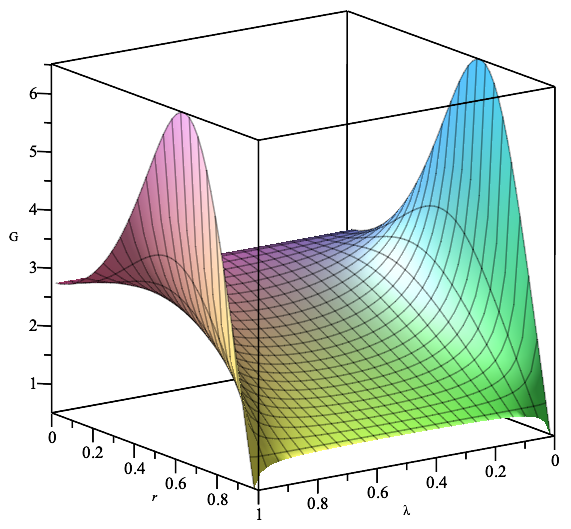
\includegraphics[width=0.65\linewidth]{Phase-Flip-Triple-Channel-Alpha=001-Beta=001-Gain-Graph.png}
\caption{Gain of Figure 34 over Figure 15 with $\alpha=0.01$ and $\beta=0.01$.}
\end{center}
\end{figure}
\newline
The gain in Figure 37 is different from that of Figure 35 and Figure 36. The purity of the initial state along with the value of $\lambda$ both have an impact for the gain of Figure 34 over Figure 15. When the initial states are pure the gain becomes zero, regardless of the value for $\lambda$. When the initial states are noisy, there is always a gain for Figure 34 over Figure 15 when $\alpha=0.01$ and $\beta=0.01$.
%---------------------------------------------------------------------------
%	Conclusion
%---------------------------------------------------------------------------
\section*{Conclusion}
It has been observed that specific scenarios produce different values for the Quantum Fisher Information and thus serve as better or worse measurement procedures. When the initial states are pure in a system the Quantum Fisher Information of product and entangled states for phase shifts can be quantified as $n$ and $n^2$ respectively. Only when initial states are pure is it more advantageous to use entangled states as measuring devices.

In the presence of phase shifts, phase flips, bit flips, and depolarization channels the Quantum Fisher Information of each measurement procedure will be different dependent upon initial conditions of the system. Phase flips tend to be less destructive when being used in measurements as compared to that of depolarization channels. In some instances with depolarization channels it is more advantageous to use noisy states than it is to use pure states. Whereas phase flips seem to be more accurate measurement procedures when the parameter is equal to one or zero.

In the example of a three particle measurement with three phase flip channels the value of each parameter is very important when it comes to calculating the Quantum Fisher Information. When the gain is calculated over the simplest phase flip scenario, if one parameter is small (parameter = 0.01) it can be shown that the gain of the three particle scenario is symmetric about the axis of another parameter (see Figures 35 and 36 for clarification). When the two parameters that are not trying to be estimated and have equal values, the purity of the initial states play a significant role in calculating the Quantum Fisher Information of a measurement.

Some scenarios have shown that it is more advantageous to use the simplest possible scenario compared to others that are more complicated. These revelations typically arise when a parameter is set to either one or zero and the purity of the state is either very low or exactly pure. The final conclusion of the research conducted in this paper should suggest that the Quantum Fisher Information of a measurement and the viability of a measurement are largely dependent upon the initial state of a system along with what is done with each system. Ideally measurements are conducted with pure states, but when noisy states are present, certain procedures such as depolarizing channels have shown to be advantageous in the pursuit of achieving precise measurements of physical parameters. 
%---------------------------------------------------------------------------
%	Bibliography
%---------------------------------------------------------------------------
\newpage
\begin{thebibliography}{99}
\bibitem{Braunstein}
Braunstein, S. L., \& Caves, C. M. (1994). Statistical distance and the geometry of quantum states. Physical Review Letters, 72(22), 3439?3443. doi: 10.1103/physrevlett.72.3439
\bibitem{Caves}
Caves, C. M. (1981). Quantum-mechanical noise in an interferometer. Physical Review D, 23(8), 1693?1708. doi: 10.1103/physrevd.23.1693
\bibitem{D. Collins}
Collins, D. (2019). Qubit-channel metrology with very noisy initial states. Physical Review A, 99(1). doi: 10.1103/physreva.99.012123
\bibitem{Hazewinkel}
Hazewinkel, M. (1995). Encyclopaedia of mathematics. an updated and annotated translation of the soviet "Mathematical encyclopaedia". Dordrecht: Kulver academic.
\bibitem{Helstrom}
Helstrom, C. W. (1969). Quantum detection and estimation theory. Journal of Statistical Physics, 1(2), 231?252. doi: 10.1007/bf01007479
\bibitem{Paris}
Paris, M. G. A. (2009). Quantum state and process estimation. Quantum Information, 139?146. doi: 10.1007/978-0-387-36944-08
\bibitem{Sarovar}
Sarovar, M., \& Milburn, G. J. (2006). Optimal estimation of one-parameter quantum channels. Journal of Physics A: Mathematical and General, 39(26), 8487?8505. doi: 10.1088/0305-4470/39/26/015
\end{thebibliography}
%-----------------------------------------------------------------------------------------------------------------------------
%	End Document
%-----------------------------------------------------------------------------------------------------------------------------
\end{document}
%---------------------------------------------------------------------------
%	Comment Headers
%---------------------------------------------------------------------------

%---------------------------------------------------------------------------
%	
%---------------------------------------------------------------------------

%--------------------------------------------------
%	
%--------------------------------------------------
